\documentclass{article}


\PassOptionsToPackage{numbers, compress}{natbib}


\usepackage[preprint]{neurips_2022}








\usepackage{xeCJK}
\usepackage{setspace}
\usepackage{caption}
\usepackage{hyperref}       %
\usepackage{url}            %
\usepackage{booktabs}       %
\usepackage{amsfonts}       %
\usepackage{nicefrac}       %
\usepackage{microtype}      %
\usepackage{xcolor}         %

\bibliographystyle{plainnat}

\usepackage{qtree}
\usepackage{latexsym}
\usepackage{microtype}
\usepackage{natbib}
\usepackage{booktabs}
\usepackage{appendix}
\usepackage{tikz}
\usepackage{tikz-dependency}
\usepackage{amsmath}
\usepackage{amsfonts}
\usepackage{graphicx}
\usepackage{amsthm}
\usepackage{mathtools}
\usepackage{multirow}
\usepackage{url}
\usepackage{color}
\usepackage{subfig}
\usepackage{dsfont}
\usepackage[ruled,vlined,noend]{algorithm2e}
\usepackage{wrapfig}
\usepackage{placeins}
\usepackage[noabbrev,capitalize]{cleveref} %
\newcommand{\crefrangeconjunction}{--}
\crefname{equation}{equation}{equations}   %
\crefname{footnote}{footnote}{footnotes}   %
\crefname{line}{line}{lines}               %
\crefname{section}{\S}{\S\S}
\Crefname{section}{\S}{\S\S}    %
\crefformat{section}{#2\S#1#3}  %
\Crefformat{section}{#2\S#1#3}
\crefrangeformat{section}{\S\S#3#1#4--#5#2#6}
\Crefrangeformat{section}{\S\S#3#1#4--#5#2#6}

\setCJKmainfont[
  BoldFont=FZHei-B01,
  ItalicFont=FZKai-Z03,
  BoldItalicFont=FZFangSong-Z02,
  SmallCapsFont=FZShuSong-Z01
]{FZShuSong-Z01}
\setCJKsansfont[AutoFakeBold=1.2, AutoFakeSlant=0.15]{FZHei-B01}
\setCJKmonofont[AutoFakeBold=1.2, AutoFakeSlant=0.15]{FZHei-B01}
\setmainfont{Times New Roman}
\setmonofont[AutoFakeBold=1.2]{LMMono10}
\setstretch{1.2}
\captionsetup{font={small,it,stretch=1.2}}

\renewcommand{\UrlFont}{\ttfamily\small}

\newcommand{\exper}[1]{\textsc{#1}}
\newcommand{\expmb}[1]{\mathbf{#1}}
\newcommand{\expobj}[1]{\mathcal{L}_\text{#1}}
\newcommand{\xx}{\expmb{x}}
\newcommand{\alphabar}{\bar{\alpha}}
\newcommand{\ww}{\expmb{w}}
\newcommand{\cc}{\expmb{c}}
\newcommand{\cx}[1]{\mathbf{x}_{#1}}
\newcommand{\ptheta}{p_\theta}
\newcommand{\mean}{\text{mean}}
\newcommand{\ptrain}{p_\text{train}}
\newcommand{\plm}{p_\text{lm}}
\newcommand{\qphi}{q_\phi}
\newcommand{\Lsimple}{\expobj{simple}}
\newcommand{\Lvlb}{\expobj{vlb}}
\newcommand{\Lsimpleee}{\mathcal{L}^\text{e2e}_\text{simple}}
\newcommand{\xstart}{\xx^{(0)}}
\newcommand{\LookUp}{\exper{LookUp}}
\newcommand{\LM}{\exper{LM}}
\newcommand{\DiffLM}{\exper{Diffusion-LM}}
\newcommand{\LMphi}{\exper{LM}_\phi}
\newcommand{\sep}{\exper{SEP}}
\newcommand{\prefix}{\exper{Prefix}}
\newcommand{\adapter}{\exper{Adapter}}
\newcommand{\FTtop}{\exper{FT-top2}}
\newcommand{\Emb}{\exper{Emb}}
\newcommand{\FT}{\exper{FT-full}}
\newcommand{\infix}{\exper{Infix}}
\newcommand{\MLP}{\exper{MLP}}
\newcommand{\yy}{\textsf{Y$_{\text{idx}}$}}
\newcommand{\pp}{\textsf{P$_{\text{idx}}$}}
\newcommand{\ppp}{\textsf{P'}}
\newcommand{\PrefixMatrix}{P}
\newcommand{\Ebare}[1][]{\mathop{\mathbb{E}}_{{#1}}}

\DeclareMathOperator{\Softmax}{softmax}
\DeclareMathOperator{\Clamp}{Clamp}
\DeclareMathOperator{\argmin}{argmin}
\DeclareMathOperator{\score}{score}
\DeclareMathOperator{\logsumexp}{logsumexp}
\newcommand\errorspan[1]{\textcolor{red}{#1}}
\newcommand\corrspan[1]{\textcolor{black}{#1}}
\newcommand\greenspan[1]{\textcolor{green}{#1}}
\newcommand\tgtspan[1]{\textbf{#1}}



\newcommand\lisa[1]{\textcolor{blue}{[Lisa: #1]}}
\newcommand\thc[1]{\textcolor{red}{[Tatsu: #1]}}
\newcommand\john[1]{\textcolor{brown}{[John: #1]}}
\newcommand\pl[1]{\textcolor{green}{[PL: #1]}}

\usepackage{microtype}


\title{Diffusion-LM 改进可控文本生成}


\author{%
  Xiang Lisa Li,  John Thickstun, Ishaan Gulrajani, Percy Liang, Tatsunori Hashimoto \\
  Computer Science Department, Stanford University\\
  \texttt{\{xlisali, jthickst,igul, thashim\}@stanford.edu}\\ \texttt{pliang@cs.stanford.edu} \\
 }

\author{%
  Xiang Lisa Li  \\
  Stanford University\\
  \texttt{xlisali@stanford.edu} \\
  \And
  John Thickstun \\
  Stanford University\\
  \texttt{jthickst@stanford.edu} \\
  \And
  Ishaan Gulrajani \\
  Stanford Univeristy \\
  \texttt{igul@stanford.edu} \\
  \And
  Percy Liang \\
  Stanford Univeristy \\
  \texttt{pliang@cs.stanford.edu} \\
  \And
  Tatsunori B. Hashimoto \\
  Stanford Univeristy \\
  \texttt{thashim@stanford.edu} \\
}


\begin{document}


\maketitle


\begin{abstract}
在不重新训练的情况下控制语言模型（LM）的行为，是自然语言生成中的一个重要开放问题。尽管近期工作已经展示了对简单句子属性（例如情感）进行控制的成功，但在复杂、细粒度控制（例如句法结构）方面进展甚微。
为应对这一挑战，我们开发了一种基于\emph{连续}扩散的新的\emph{非自回归}语言模型，称为 Diffusion-LM。
基于扩散模型在连续域中的近期成功，Diffusion-LM 迭代地将一系列 Gaussian 向量去噪为词向量，从而产生一系列中间隐变量。
这些中间变量的连续、层次化性质，使一种简单的基于梯度的算法能够执行复杂的可控生成任务。
我们在六个具有挑战性的细粒度控制任务上展示了对 Diffusion-LM 的成功控制，并显著优于先前工作。\footnote{代码可在 \url{https://github.com/XiangLi1999/Diffusion-LM.git} 获取。}
\end{abstract}

\section{引言}
\label{sec:intro}

大型自回归语言模型（LM）能够生成高质量文本 \cite{radford2019language,brown-et-al-gpt3,Chowdhery2022PaLMSL,Zhang2022OPT}，但为了在真实世界应用中可靠地部署这些 LM，文本生成过程需要是\emph{可控的}：我们需要生成满足期望要求（例如主题、句法结构）的文本。
控制 LM 的一种自然方法，是使用 (control, text) 形式的监督数据对 LM 进行微调
\cite{Keskar2019CTRL}。然而，为每个控制任务更新 LM 参数可能代价高昂，并且不允许组合多个控制（例如生成既具有正向情感\emph{又}无毒的文本）。
这促使人们采用轻量且模块化的 plug-and-play 方法 \cite{Dathathri2020Plug}：保持 LM 冻结，并使用外部分类器引导生成过程，该分类器衡量生成文本满足控制的程度。
但是，引导冻结的自回归 LM 已被证明是困难的，而已有成功仅限于
简单的属性级控制（例如情感或主题）\cite{Dathathri2020Plug,KrauseGeDi2020,yang-klein-2021-fudge}。

为处理更复杂的控制，
我们提出\emph{Diffusion-LM}，一种基于\emph{连续}扩散的新的语言模型。
如 \cref{fig:1} 所示，Diffusion-LM 从一系列 Gaussian 噪声向量开始，并逐步将其去噪为与词对应的向量。
这些渐进去噪步骤产生了连续隐表征的层次结构。
我们发现，这种层次化且连续的隐变量使简单的基于梯度的方法能够执行复杂控制任务，例如约束生成序列的解析树。



\begin{figure}
    \centering
    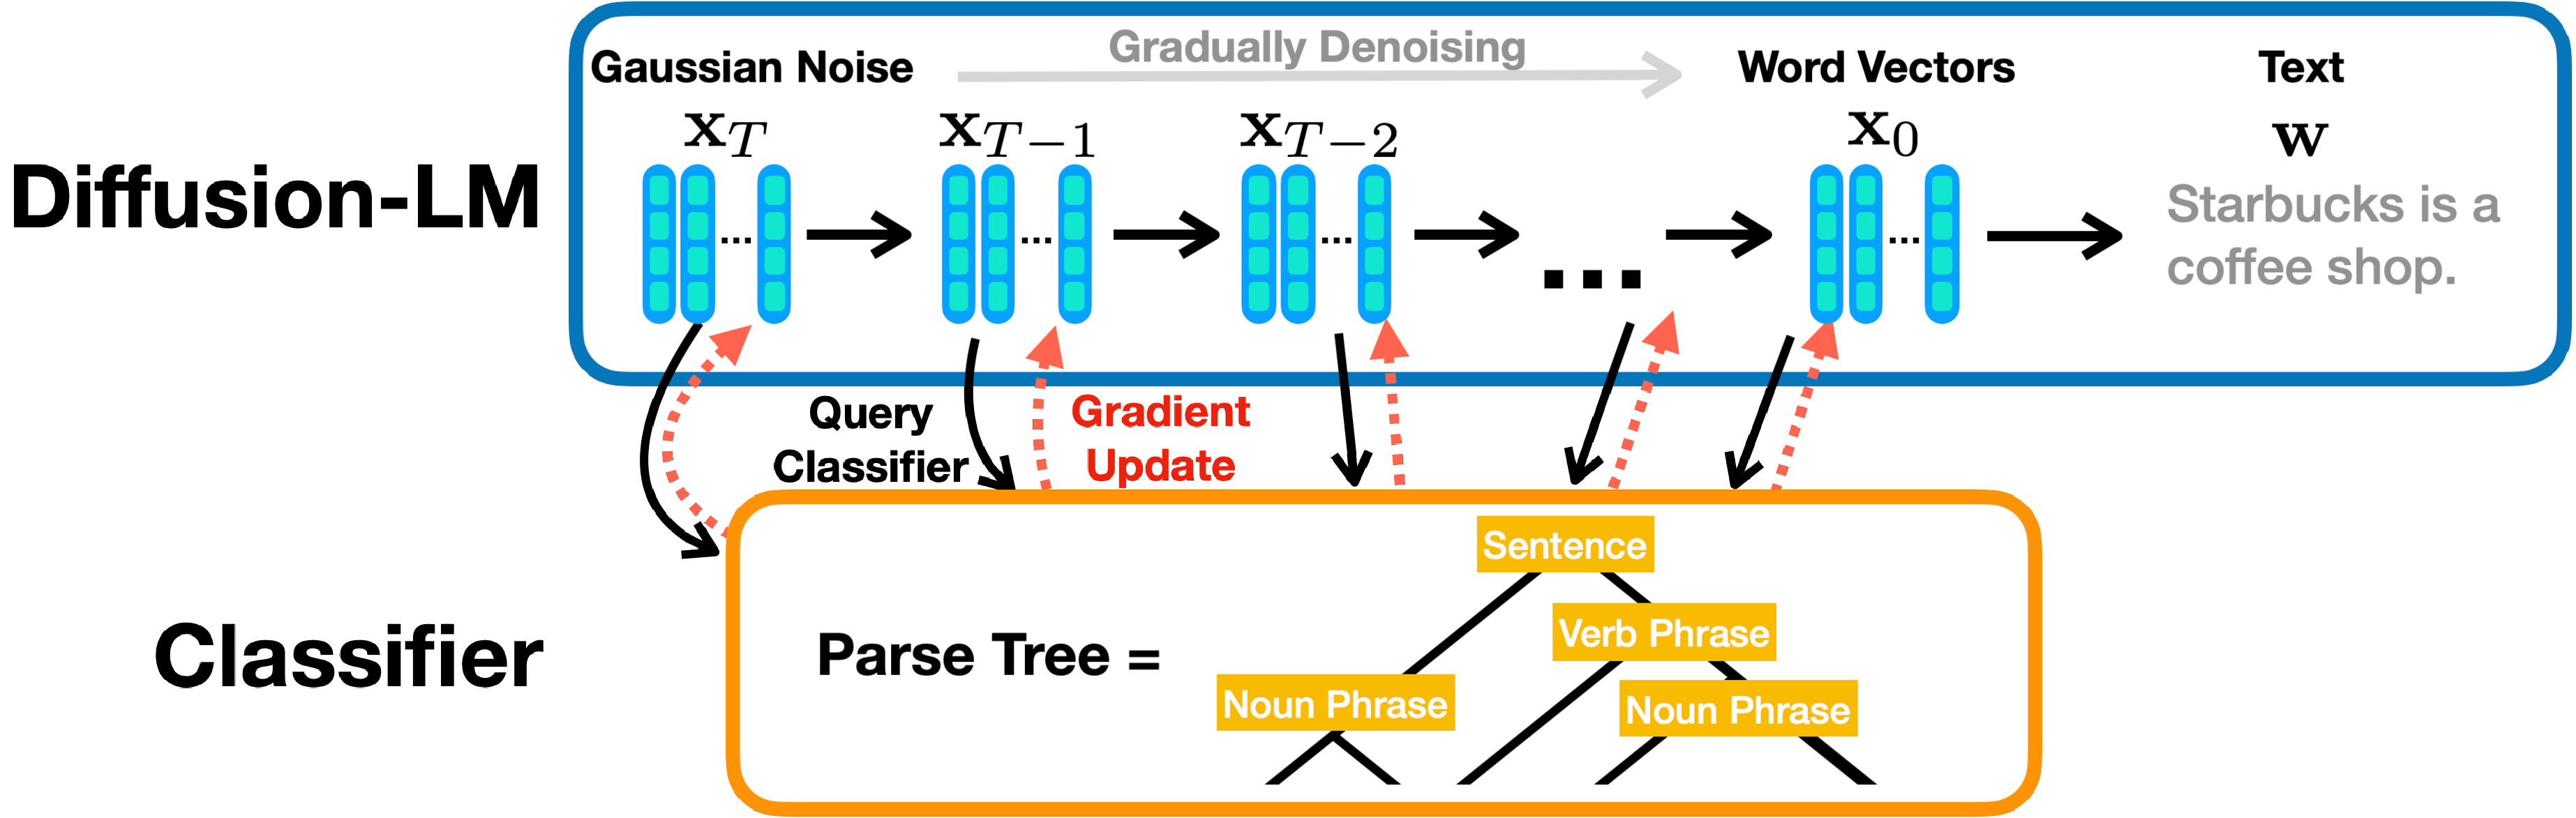
\includegraphics[width=0.8\textwidth]{fig/fig1_v2.pdf}
     \caption{\label{fig:1} Diffusion-LM 迭代地将一系列 Gaussian 向量去噪为词向量，产生噪声水平递减的中间隐变量 $\cx{T} \cdots \cx{0}$。对于可控生成，我们在这些连续隐变量上迭代执行梯度更新，以优化流畅性（由 Diffusion-LM 参数化）并满足控制要求（由分类器参数化）。
     \vspace{-5mm}
    }
\end{figure}


连续扩散模型在视觉和音频领域取得了极大成功 \cite{ho2020denoising,kong2020diffwave,ramesh2022hierarchical,dhariwal2021diffusion,chen2021wavegrad}，但由于文本固有的离散性质，它们尚未应用于文本（\cref{sec:background}）。将这类模型适配到文本需要对标准扩散进行若干修改：我们向标准扩散过程添加 embedding 步骤和 rounding 步骤，设计训练目标来学习 embedding，并提出改进 rounding 的技术（\cref{sec:method}）。
如 \cref{fig:1} 所示，我们使用基于梯度的方法控制 Diffusion-LM。该方法使我们能够将文本生成过程引导到满足目标结构和语义控制的输出。它在 Diffusion-LM 的连续隐变量上迭代执行梯度更新，以平衡流畅性与控制满足度（\cref{ssec:control_text}）。%

为展示 Diffusion-LM 的可控性，我们考虑六个控制目标，范围从细粒度属性（例如语义内容）到复杂结构（例如解析树）。
在所有这些分类器引导的控制任务上，我们的方法几乎将先前 plug-and-play 方法的成功率翻倍，并达到或优于微调 oracle（\cref{ssec:control}）。
除了这些单独的控制任务外，我们还表明，可以成功组合多个分类器引导的控制，生成同时具有期望语义内容和句法结构的句子（\cref{ssec:compose}）。
最后，我们考虑 span-anchored 控制，例如长度控制和 infilling。Diffusion-LM 允许我们\emph{无需}分类器即可执行这些控制任务，并且我们的 Diffusion-LM 显著优于先前 plug-and-play 方法，在 infilling 任务上与从头训练的自回归 LM 相当（\cref{ssec:infill}）。

\section{相关工作}
\label{sec:related_work}


\paragraph{文本扩散模型。}
扩散模型 \cite{pmlr-v37-sohl-dickstein15} 已在连续数据域中展示出巨大成功 \cite{ho2020denoising,nichol2021improved, kong2020diffwave, Mittal2021Music}，能够生成具有 state-of-the-art 样本质量的图像和音频。为处理离散数据，过去工作研究了\emph{离散}状态空间上的文本扩散模型，在离散数据上定义加噪过程（例如，每个 token 有一定概率被加噪为吸收或随机 token）\cite{austin2021structured,hoogeboom2021argmax,hoogeboom2022autoregressive}。
本文聚焦于文本的\emph{连续}扩散模型；据我们所知，我们的工作是首个探索这一设定的工作。
与离散扩散 LM 相比，我们的连续扩散 LM 诱导连续隐表征，使高效的基于梯度的方法能够用于可控生成。

\paragraph{自回归与非自回归 LM。}
大多数大型预训练 LM 都是从左到右的自回归模型（例如 GPT-3 \cite{brown-et-al-gpt3}、PaLM \cite{Chowdhery2022PaLMSL}）。固定的生成顺序限制了模型在许多可控生成设定中的灵活性，尤其是那些
对左右上下文全局施加控制的设定。一个例子是 infilling，它对右上下文施加词汇控制；另一个例子是句法结构控制，它控制涉及左右上下文的全局属性。
由于自回归 LM 不能直接以右上下文为条件，先前工作为这些任务开发了专门的训练和解码技术 \cite{sha-2020-gradient,donahue-etal-2020-enabling,qin-etal-2020-back}。
例如，\citet{Qin-COLD} 提出了一种解码方法，将离散 LM 输出松弛为连续变量，并从右上下文反向传播梯度信息。
Diffusion-LM 可以以任意分类器为条件，这些分类器可考察句子的复杂全局属性。
也有其他非自回归 LM 被开发用于机器翻译和 speech-to-text 任务 \cite{gu2018nonautoregressive,saharia2020latentalignments}。
然而，这些方法专门面向语音和翻译设定，其中有效输出上的熵较低，
并且已有研究表明这些方法在语言建模上失败 \cite{ren-etal-2020-study}。

\paragraph{Plug-and-Play 可控生成。}
Plug-and-play 可控生成旨在保持 LM 冻结，并使用势函数（例如分类器）引导其输出。给定一个衡量生成文本满足期望控制程度的概率势函数，生成文本应同时针对控制满足度（由势函数衡量）和流畅性（由 LM 概率衡量）进行优化。
有若干基于自回归 LM 的 plug-and-play 方法：
FUDGE \cite{yang-klein-2021-fudge} 用部分序列控制满足度的估计，对每个 token 处的 LM 预测重新加权；
GeDi \cite{KrauseGeDi2020} 和 DExperts \cite{liu-etal-2021-dexperts} 使用为控制任务微调/训练的较小 LM，对每个 token 处的 LM 预测重新加权。


与我们最接近的工作是 PPLM \cite{Dathathri2020Plug}，它在自回归 LM 的隐藏激活上执行梯度上升，以引导 next-token 满足控制并保持流畅性。
由于 PPLM 基于自回归 LM，它只能从左到右生成。这阻止了 PPLM 修复和恢复先前生成步骤中产生的错误。
尽管这些方法在属性（例如主题）控制上取得成功，但我们将在 \cref{ssec:control} 中表明，这些用于自回归 LM 的 plug-and-play 方法在更复杂的控制任务上会失败，例如控制句法结构和语义内容。我们通过对 Diffusion-LM 诱导的连续隐变量序列应用分类器引导的梯度更新，证明 Diffusion-LM 能够进行 plug-and-play 可控生成。




\newcommand{\xxtheta}{f_\theta} 
\section{问题陈述与背景}
\label{sec:background}

我们首先定义可控生成（\cref{ssec:control_setup}），随后回顾连续扩散模型（\cref{ssec:diffusion_setup}）。

\subsection{文本生成模型与可控生成} 
\label{ssec:control_setup}
文本生成的任务是从已训练的语言模型 $\plm (\ww)$ 中采样 $\ww$，其中 $\ww = [w_1 \cdots w_n]$ 是离散词序列，$\plm (\ww)$ 是词序列上的概率分布。可控文本生成的任务是从条件分布 $p(\ww \mid \cc)$ 中采样 $\ww$，其中 $\cc$ 表示一个\emph{控制}变量。对于句法控制，$\cc$ 可以是目标句法树（\cref{fig:1}）；对于情感控制，$\cc$ 可以是期望的情感标签。可控生成的目标是生成满足控制目标 $\cc$ 的 $\ww$。

考虑 plug-and-play 可控生成设定：给定一个由大量无标注文本数据训练得到的语言模型 $\plm(\ww)$，并且对于每个控制任务，给定一个由较少量有标注文本数据训练得到的分类器 $p(\cc \mid \ww)$（例如，对于句法控制，该分类器是概率解析器）。目标是利用这两个模型，通过 Bayes 规则 $p(\ww \mid \cc) \propto \plm(\ww) \cdot p(\cc \mid \ww)$ 从后验 $p(\ww \mid \cc)$ 中近似采样。这里，$\plm(\ww)$ 鼓励 $\ww$ 保持流畅，而 $p(\cc \mid \ww)$ 鼓励 $\ww$ 满足控制。






\subsection{自回归语言模型}
语言建模的典型方法以从左到右的自回归方式分解 $\plm$，即 $\plm(\ww) = \plm(w_1) \prod_{i=2}^n \plm(x_i \mid x_{<i})$。在这种情况下，文本生成被化约为在已生成部分序列条件下反复预测 next-token 的任务。next-token 预测 $\plm(x_i \mid x_{<i})$ 通常由 Transformer 架构 \cite{Vaswani2017Attn} 参数化。

\subsection{连续域的扩散模型}
\label{ssec:diffusion_setup}

扩散模型 \citep{ho2020denoising,nichol2021improved} 是一种隐变量模型，它将数据 $\cx{0} \in \mathbb{R}^d$ 建模为 Markov 链 $\cx{T} \dots \cx{0}$，其中每个变量都在 $\mathbb{R}^d$ 中，且 $\cx{T}$ 是 Gaussian。扩散模型逐步对隐变量序列 $\cx{T:1}$ 去噪，以近似来自目标数据分布的样本~（\cref{fig:graphical_model}）。初始状态 $p_\theta(\cx{T}) \approx \mathcal{N} (0, \mathbf{I})$，每个去噪转移 $\cx{t} \rightarrow \cx{t-1}$ 由模型 $\ptheta(\cx{t-1}\mid \cx{t}) = \mathcal{N}(\cx{t-1}; \mu_\theta(\cx{t}, t), \Sigma_\theta(\cx{t}, t))$ 参数化。例如，$\mu_\theta$ 和 $\Sigma_\theta$ 可由 U-Net 或 Transformer 计算得到。


为了训练扩散模型，我们定义一个构造中间隐变量 $\cx{1:T}$ 的前向过程。前向过程逐步向数据 $\cx{0}$ 添加 Gaussian 噪声，直到在扩散步骤 $T$ 时样本 $\cx{T}$ 近似为 Gaussian。每个转移 $\cx{t-1} \rightarrow \cx{t}$ 由 $q(\cx{t} \mid \cx{t-1}) = \mathcal{N} (\cx{t} ; \sqrt{1-\beta_t} \cx{t-1}, \beta_t \mathbf{I})$ 参数化，其中超参数 $\beta_t$ 是扩散步骤 $t$ 添加的噪声量。
前向过程 $q$ 的这种参数化不包含可训练参数，并使我们能够定义一个训练目标：按照预定义的前向过程 $q$ 生成带噪数据，并训练模型反转该过程以重构数据。




\begin{figure}
    \centering
    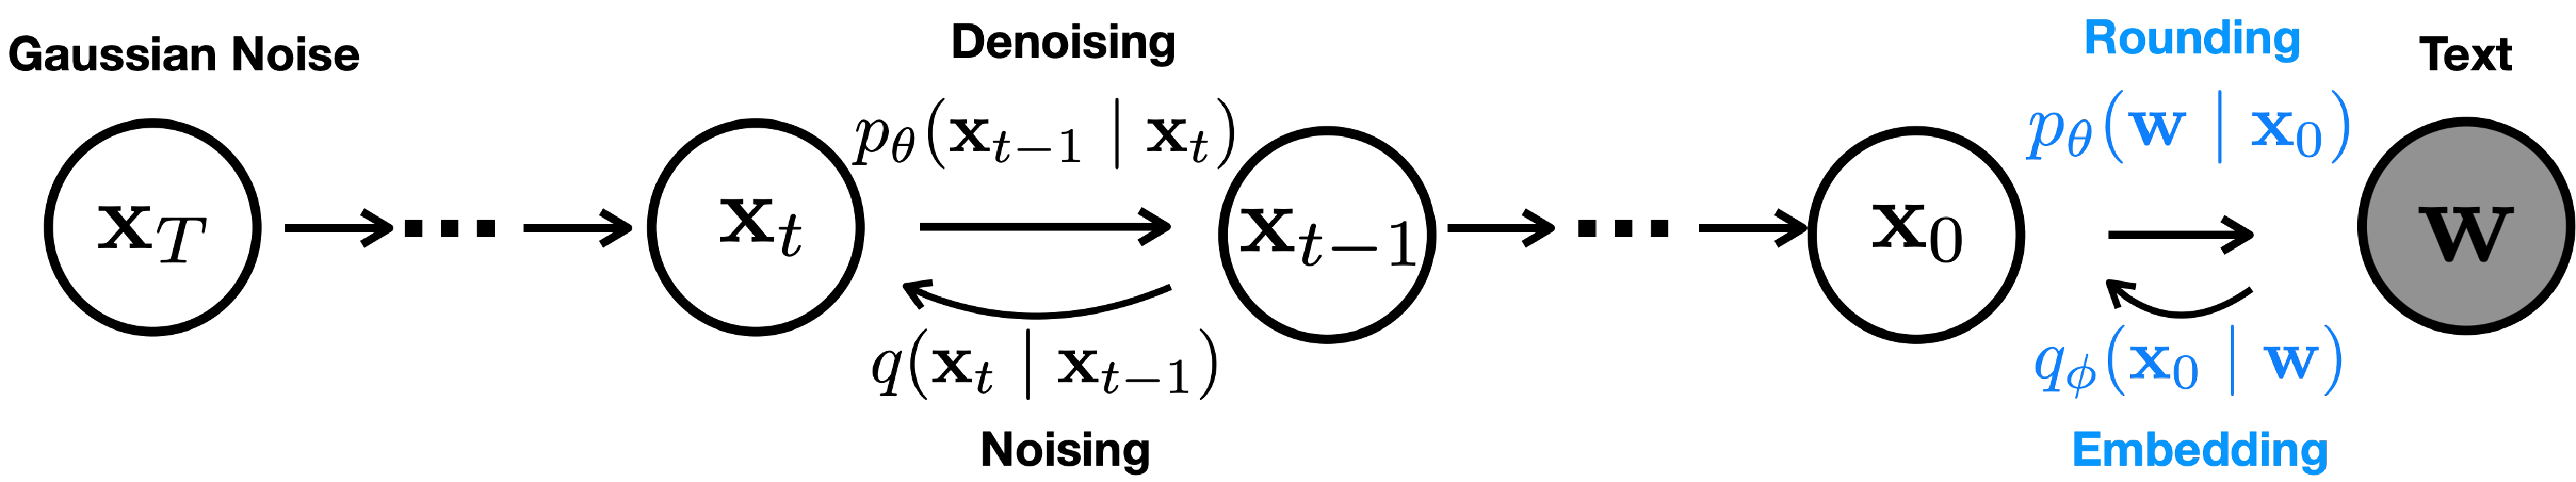
\includegraphics[width=0.8\textwidth]{fig/graphical_model_v2.pdf}
    \caption{\label{fig:graphical_model} 表示前向和反向扩散过程的图模型。除原始扩散模型 \cite{ho2020denoising} 外，我们在 $\cx{0}$ 与 $\ww$ 之间加入一个 Markov 转移，并提出 embedding \cref{ssec:embeddings} 和 rounding \cref{ssec:rounding} 技术。}
    \vspace{-5mm}
\end{figure}

扩散模型通过最大化数据的边际似然 $\mathbb{E}_{\cx{0} \sim p_\text{data} }[\log p_\theta(\cx{0})]$ 进行训练，其典型目标是 $\log p_\theta(\cx{0})$ 的变分下界 \cite{pmlr-v37-sohl-dickstein15}，
\begin{equation}
\Lvlb (\cx{0}) = \mathop{\mathbb{E}}_{q(\cx{1:T} | \cx{0})} \left[\log \frac{q(\cx{T} | \cx{0})}{\ptheta(\cx{T})} + \sum_{t=2}^T \log \frac{q(\cx{t-1} | \cx{0},\cx{t})} {\ptheta(\cx{t-1} | \cx{t}) } - \log \ptheta( \cx{0} | \cx{1})\right].
\label{eqn:diffusion}
\end{equation}
然而，该目标可能不稳定，并且需要许多优化技巧来稳定训练 \cite{nichol2021improved}。为规避这一问题，\citet{ho2020denoising} 设计了一个简单的替代目标，对 $\Lvlb$ 中每个 KL-divergence 项进行展开并重新加权，从而得到均方误差损失（推导见 \cref{app:derive}），我们将其记为
\[\Lsimple (\cx{0}) = \sum_{t=1}^T \mathop{\mathbb{E}}_{q(\cx{t} \mid \cx{0})} || \mu_\theta(\cx{t}, t) - \hat{\mu}(\cx{t}, \cx{0}) ||^2,\]
其中 $\hat{\mu}(\cx{t}, \cx{0})$ 是后验 $q(\cx{t-1} | \cx{0},\cx{t})$ 的均值，该后验是闭式 Gaussian；$\mu_\theta(\cx{t}, t)$ 是由神经网络计算得到的 $\ptheta(\cx{t-1} \mid \cx{t})$ 的预测均值。
虽然 $\Lsimple$ 不再是有效下界，但先前工作发现它在经验上使训练更稳定并提高了样本质量\footnote{我们这里对 $\Lsimple$ 的定义使用了与 \citet{ho2020denoising} 不同的参数化。我们用 $\mu_\theta(\cx{t}, t)$ 表示平方损失，而他们用 $\epsilon_\theta(\cx{t}, t)$ 表示。}。
我们将在 Diffusion-LM 中使用类似的简化，以稳定训练并提升样本质量（\cref{ssec:embeddings}）。














\vspace{-2mm}
\section{Diffusion-LM：连续扩散语言建模}
\vspace{-2mm}
\label{sec:method}

构建 Diffusion-LM 需要对标准扩散模型进行若干修改。
首先，我们必须定义一个 embedding 函数，将离散文本映射到连续空间。为此，我们提出一个用于学习 embeddings 的端到端训练目标（\cref{ssec:embeddings}）。
其次，我们需要一种 rounding 方法，将 embedding 空间中的向量映射回词。为此，我们提出训练和解码阶段的方法以促进 rounding（\cref{ssec:rounding}）。








\vspace{-2mm}
\subsection{端到端训练} 
\label{ssec:embeddings}


为将连续扩散模型应用于离散文本，我们定义 embedding 函数 $\Emb(w_i)$，将每个词映射到 $\mathbb{R}^{d}$ 中的向量。我们将长度为 $n$ 的序列 $\ww$ 的 embedding 定义为：$\Emb(\ww) = [\Emb(w_1), \dots, \Emb(w_n)] \in \mathbb{R}^{nd}$。

我们提出对扩散模型训练目标（Equation \ref{eqn:diffusion}）的修改，以联合学习扩散模型的参数和词 embeddings。
在初步实验中，我们探索了随机 Gaussian embeddings 以及预训练词 embeddings \cite{pennington-etal-2014-glove, radford2019language}。我们发现，与端到端训练相比，这些固定 embeddings 对 Diffusion-LM 而言是次优的\footnote{尽管可训练 embeddings 在控制和生成任务上表现最佳，但我们发现，在优化 held-out 困惑度时，映射到词表单纯形上的固定 embeddings 是有帮助的。由于本文关注生成质量而非困惑度，我们将该方法与困惑度结果的讨论留到 \cref{app:simplex}。}。


如 Figure \ref{fig:graphical_model} 所示，我们的方法在前向过程中加入从离散词 $\ww$ 到 $\cx{0}$ 的 Markov 转移，由 $\qphi(\cx{0} | \ww) = \mathcal{N} (\Emb(\ww), \sigma_0 I )$ 参数化。在反向过程中，我们加入一个可训练的 rounding 步骤，由 $\ptheta(\ww \mid \cx{0}) = \prod_{i=1}^n \ptheta(w_i \mid x_i)$ 参数化，其中 $\ptheta(w_i \mid x_i)$ 是 softmax 分布。\cref{sec:background} 中引入的训练目标现在变为
\begin{equation}
\begin{aligned}
\mathcal{L}^\text{e2e}_{\text{vlb}} (\ww) &= \mathop{\mathbb{E}}_{q_\phi(\cx{0} | \ww)}\left[\mathcal{L}_{\text{vlb}} (\cx{0}) + \log \qphi(\cx{0} | \ww) - \log \ptheta(\ww | \cx{0})]\right], \\
 \mathcal{L}^\text{e2e}_\text{simple} (\ww) &= \mathop{\mathbb{E}}_{\qphi(\cx{0:T} | \ww)} \left[\Lsimple(\cx{0}) + || \Emb(\ww) - \mu_\theta(\cx{1}, 1) ||^2  - \log \ptheta(\ww | \cx{0})\right].
\end{aligned}
\label{obj:e2e}
\end{equation}
\begin{wrapfigure}[11]{R}{0.5\textwidth}
\vspace{-10mm}
\centering
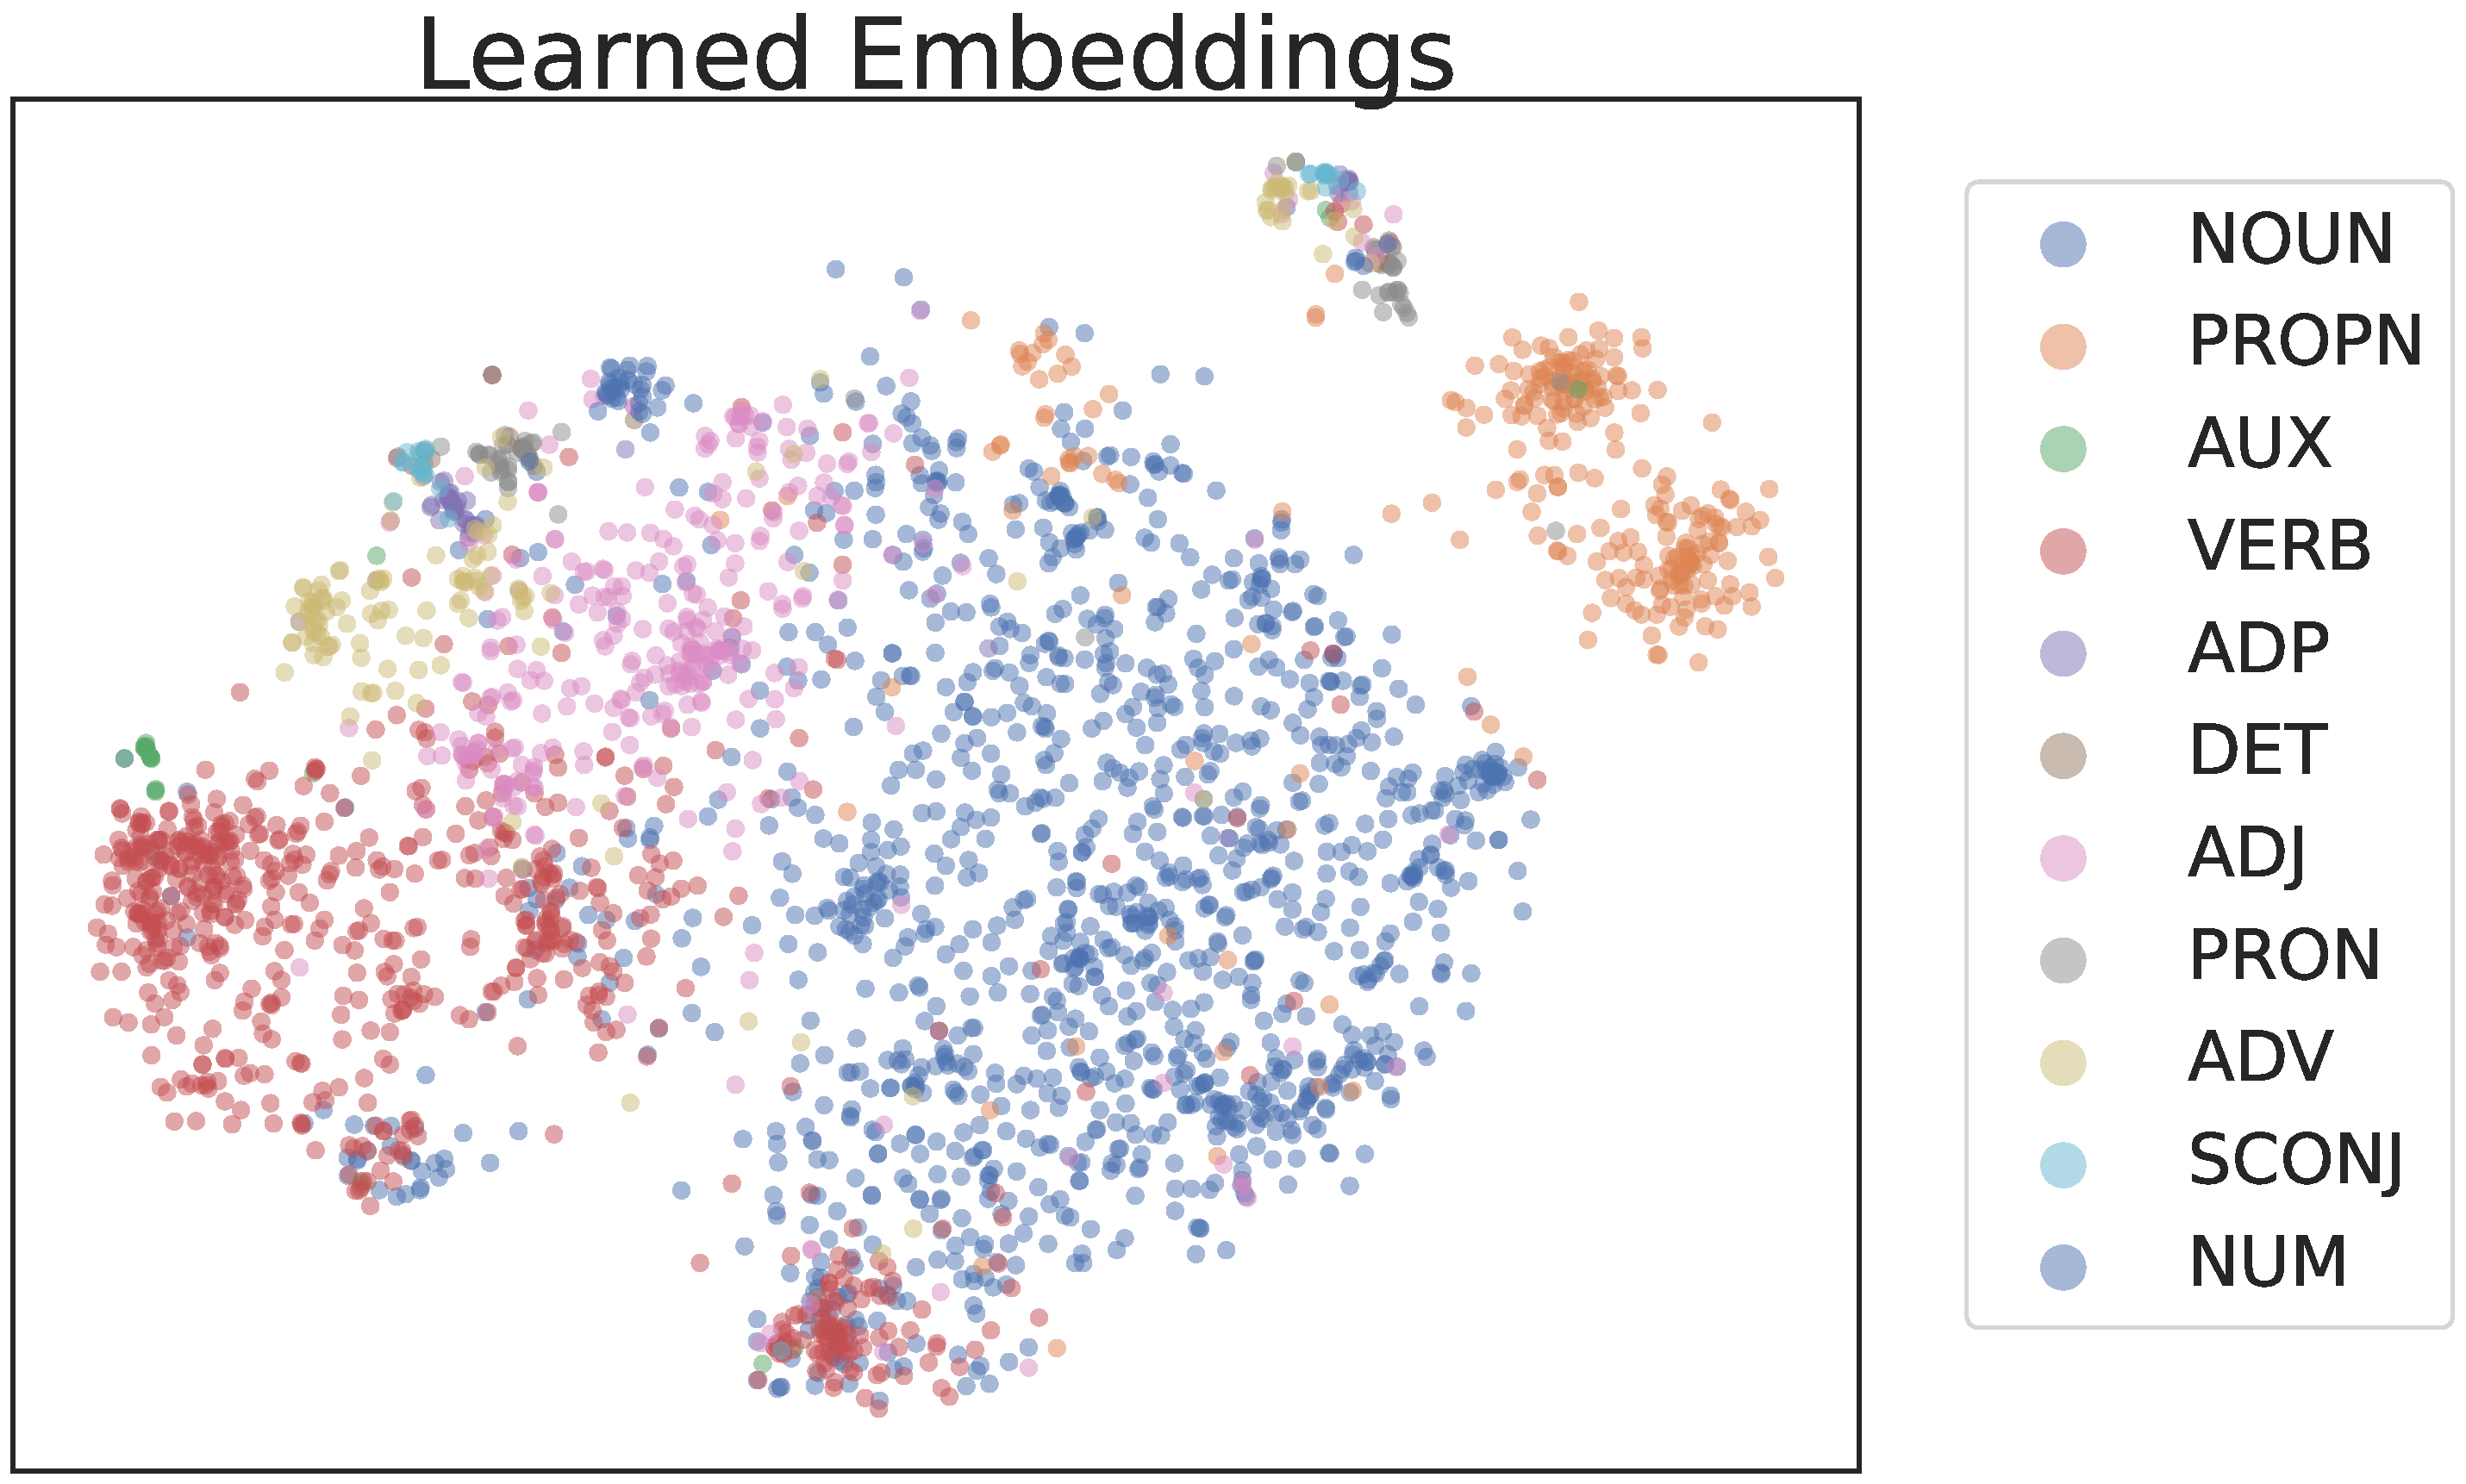
\includegraphics[width=\linewidth]{fig/embedding_128_v3.pdf}\caption{ \label{fig:emb} 学到的词 embeddings 的 t-SNE \cite{vanDerMaaten2008} 图。每个词按其 POS 着色。\looseness=-1 }
\end{wrapfigure}

我们遵循 \cref{ssec:diffusion_setup} 中的简化，从 $\mathcal{L}^\text{e2e}_{\text{vlb}}(\ww)$ 推导 $ \mathcal{L}^\text{e2e}_\text{simple} (\ww)$，推导细节见 \cref{app:derive}。由于我们正在训练 embedding 函数，$q_\phi$ 现在包含可训练参数，因此我们使用重参数化技巧 \citep{rezende2014stochastic, kingma2014auto} 通过该采样步骤进行反向传播。
经验上，我们发现学到的 embeddings 形成有意义的聚类：具有相同 part-of-speech 标签（句法角色）的词倾向于聚在一起，如 \cref{fig:emb} 所示。



\subsection{减少 Rounding 错误}
\label{ssec:rounding}


学到的 embeddings 定义了从离散文本到连续 $\cx{0}$ 的映射。我们现在描述其逆过程，即将预测的 $\cx{0}$ rounding 回离散文本。Rounding 通过根据 argmax $\ptheta(\ww \mid \cx{0})= \prod_{i=1}^n \ptheta(w_i \mid x_i)$ 为每个位置选择概率最高的词来实现。理想情况下，这种 argmax-rounding 足以映射回离散文本，因为去噪步骤应确保 $\cx{0}$ 精确落在某个词的 embedding 上。然而在经验上，模型无法生成承诺于单个词的 $\cx{0}$。



这一现象的一种解释是，我们目标 \ref{obj:e2e} 中的 $\Lsimple(\cx{0})$ 项对 $\cx{0}$ 结构建模的强调不足。回忆我们定义 $\Lsimple(\cx{0}) =\sum_{t=1}^T \mathbb{E}_{\cx{t}}|| \mu_\theta(\cx{t}, t) - \hat{\mu}(\cx{t}, \cx{0}) ||^2$，其中我们的模型 $\mu_\theta(\cx{t}, t)$ 在每个去噪步骤 $t$ 直接预测 $\ptheta(\cx{t-1}\mid \cx{t})$ 的均值。
在该目标中，$\cx{0}$ 必须承诺于单个词 embedding 的约束只会出现在 $t$ 接近 $0$ 的项中；我们发现，这种参数化需要仔细调参才能迫使目标强调这些项（见 \cref{app:ablation}）。


\newcommand{\Lsimplexx}{\mathcal{L}^\text{e2e}_{\cx{0}\text{-simple}}}
我们的方法对 $\Lsimple$ 重新参数化，迫使 Diffusion-LM 在目标的\emph{每一}项中显式建模 $\cx{0}$。具体而言，我们推导了一个通过 $\cx{0}$ 参数化的 $\Lsimple$ 类似形式，
$\Lsimplexx(\cx{0})=\sum_{t=1}^T \mathbb{E}_{\cx{t}} ||\xxtheta(\cx{t}, t) - \cx{0} ||^2$，其中我们的模型 $\xxtheta(\cx{t}, t)$ 直接预测 $\cx{0}$\footnote{预测 $\cx{0}$ 与预测 $\cx{t-1}$ 只相差缩放常数，因为 $\cx{t-1}$ 的分布可通过前向过程 $\cx{t-1} = \sqrt{\alphabar} \cx{0} +\sqrt{1-\alphabar} \epsilon$ 以闭式获得，更多细节见 \cref{app:derive}。}。这迫使神经网络在每一项中预测 $\cx{0}$，并且我们发现，用该目标训练的模型会很快学到 $\cx{0}$ 应精确地位于某个词 embedding 的中心。

我们已经说明重新参数化如何有助于模型训练，但我们也发现，同一直觉可在解码时用于一种称为\emph{clamping} 技巧的方法。
对于 $\cx{0}$-参数化模型的标准生成方法，模型先通过 $\xxtheta(\cx{t}, t)$ 计算 $\cx{0}$ 的估计，然后在该估计条件下采样 $\cx{t-1}$，从而将 $\cx{t}$ 去噪为 $\cx{t-1}$：$\cx{t-1} = \sqrt{\alphabar} \xxtheta(\cx{t}, t) +\sqrt{1-\alphabar} \epsilon$，其中 $\alphabar_t = \prod_{s=0}^t (1-\beta_s)$ 且 $\epsilon \sim \mathcal{N}(0,I)$\footnote{这来自边缘分布 $q(\cx{t} \mid \cx{0})$，由于所有 Markov 转移都是 Gaussian，该分布具有闭式形式。}。在 clamping 技巧中，模型还会将预测向量 $\xxtheta(\cx{t}, t)$ 映射到最近的词 embedding 序列。此时，采样步骤变为 $\cx{t-1} = \sqrt{\alphabar}\cdot \Clamp(\xxtheta(\cx{t}, t)) +\sqrt{1-\alphabar} \epsilon$。Clamping 技巧迫使预测向量在中间扩散步骤承诺于某个词，使向量预测更精确并减少 rounding 错误。\footnote{直观上，在 $t$ 接近 $T$ 的早期扩散步骤应用 clamping 技巧可能是次优的，因为模型尚未确定要承诺于哪些词。经验上，对所有扩散步骤应用 clamping 技巧不会显著损害性能。但遵循这一直觉，也可以将 clamping 技巧的起始步骤设为超参数。}
















\section{使用 Diffusion-LM 进行解码与可控生成}
\label{sec:decode}
在描述 Diffusion-LM 之后，我们现在考虑可控文本生成（\cref{ssec:control_text}）和解码（\cref{ssec:mbr1}）问题。


\subsection{可控文本生成}
\label{ssec:control_text}
我们现在描述一种在 Diffusion-LM 上实现 plug-and-play 控制的过程。我们的控制方法受到 \cref{ssec:control_setup} 中 Bayesian 形式化的启发，但并不直接在离散文本上进行控制，而是在 Diffusion-LM 定义的连续隐变量序列 $\cx{0:T}$ 上进行控制，并应用 rounding 步骤将这些隐变量转换为文本。

控制 $\cx{0:T}$ 等价于从后验 $p(\cx{0:T} | \cc) = \prod_{t=1}^T p(\cx{t-1} \mid \cx{t}, \cc)$ 解码，并且我们将该联合推理问题分解为每个扩散步骤上的一系列控制问题：$p(\cx{t-1} \mid \cx{t}, \cc) \propto p(\cx{t-1} \mid \cx{t}) \cdot p(\cc \mid \cx{t-1}, \cx{t})$。
进一步地，我们依据先前控制扩散工作的条件独立假设 \cite{song2021scorebased}，将 $p(\cc \mid \cx{t-1}, \cx{t})=p(\cc \mid \cx{t-1})$ 简化。因此，对于第 $t$ 步，我们在 $\cx{t-1}$ 上执行梯度更新：
\begin{align*}
    \nabla_{\cx{t-1}} \log p(\cx{t-1} \mid \cx{t}, \cc) = \nabla_{\cx{t-1}} \log p(\cx{t-1} \mid \cx{t}) + \nabla_{\cx{t-1}}  \log  p(\cc \mid \cx{t-1}),
\end{align*}
其中 $\log p(\cx{t-1} \mid \cx{t})$ 和 $\log p(\cc \mid \cx{t-1})$ 都是可微的：第一项由 Diffusion-LM 参数化，第二项由神经网络分类器参数化。


类似于图像设定中的工作 \cite{dhariwal2021diffusion,song2021scorebased}，我们在扩散隐变量上训练分类器，并在隐空间 $\cx{t-1}$ 上执行梯度更新，以引导其满足控制。这些图像扩散工作在每个扩散步骤沿 $\nabla_{ \cx{t-1}} \log  p(\cc \mid \cx{t-1})$ 方向走一步梯度。为提升文本上的性能并加速解码，我们引入两个关键修改：流畅性正则化和多步梯度更新。\looseness=-1




为生成流畅文本，我们在带有\emph{流畅性正则化}的控制目标上执行梯度更新：$ \lambda \log p(\cx{t-1} \mid \cx{t}) + \log p(\cc \mid \cx{t-1})$，其中 $\lambda$ 是在流畅性（第一项）与控制（第二项）之间权衡的超参数。尽管现有的扩散可控生成方法未在目标中包含 $\lambda \log p(\cx{t-1} \mid \cx{t})$ 项，我们发现该项对于生成流畅文本至关重要。所得可控生成过程可视为一种随机解码方法，它在最大化与采样 $p(\cx{t-1} \mid \cx{t}, \cc)$ 之间取得平衡，这很像 nucleus sampling~\cite{Holtzman2020Nucleus} 或低温采样等流行文本生成技术。为提升控制质量，我们对每个扩散步骤执行多步梯度更新：对每个扩散步骤运行 $3$ 步 Adagrad\footnote{我们尝试了将 Adagrad 替换为 SGD 的消融，但发现 Adagrad 对超参数调节明显不那么敏感。} \cite{Duchi2010AdaptiveSM} 更新。为缓解增加的计算成本，我们将扩散步骤从 2000 下采样到 200，这能加速我们的可控生成算法且不会显著损害样本质量。


\subsection{最小 Bayes 风险解码}
\label{ssec:mbr1}
许多条件文本生成任务需要一个\emph{单一}的高质量输出序列，例如机器翻译或句子 infilling。
在这些设定中，我们应用 Minimum Bayes Risk (MBR) 解码 \cite{kumar-byrne-2004-minimum} 来聚合从 Diffusion-LM 抽取的一组样本 $\mathcal{S}$，并选择在损失函数 $\mathcal{L}$（例如负 BLEU 分数）下达到最小期望风险的样本：$\hat{\ww} = \argmin_{\ww \in S} \sum_{\ww' \in S} \frac{1}{|S|}\mathcal{L}(\ww, \ww')$。我们发现 MBR 解码通常会返回高质量输出，因为低质量样本会与其余样本不相似，并受到损失函数惩罚。








\newcommand{\Length}{Length\xspace}
\newcommand{\Spans}{Syntax Spans\xspace} 
\newcommand{\POS}{Parts-of-speech\xspace}
\newcommand{\Syntax}{Syntax Tree\xspace} 
\newcommand{\Content}{Semantic Content\xspace} 

\section{实验设置}
通过上述对训练（\cref{sec:method}）和解码（\cref{sec:decode}）的改进，我们为两个语言建模任务训练 Diffusion-LM。随后，我们将可控生成方法应用于 $5$ 个分类器引导的控制任务，并将 MBR 解码应用于一个无分类器控制任务（即 infilling）。

\label{sec:setup}
\subsection{数据集与超参数} 
我们在两个数据集上训练 Diffusion-LM：E2E \cite{novikova-etal-2017-e2e} 和 ROCStories \cite{mostafazadeh-etal-2016-corpus}。E2E 数据集包含 50K 条餐馆评论，这些评论由 8 个字段标注，包括食物类型、价格和顾客评分。
ROCStories 数据集包含 98K 个五句故事，
捕获了日常事件之间丰富的因果和时间常识关系。
该数据集比 E2E 更难建模，因为故事包含更大的 11K 词词表和更丰富的语义内容。


我们的 Diffusion-LM 基于具有 $80$M 参数的 Transformer \cite{Vaswani2017Attn} 架构，序列长度为 $n=64$，扩散步骤为 $T=2000$，并采用平方根噪声调度（详见 \cref{app:noise}）。我们将 embedding 维度视为超参数，对 E2E 设为 $d=16$，对 ROCStories 设为 $d=128$。超参数细节见 \cref{app:hyperparam}。
在解码时，我们对 E2E 下采样到 200 个扩散步骤，对 ROCStories 保持 2000 个步骤。使用 200 步解码 Diffusion-LM 仍比解码自回归 LM 慢 7 倍。对于可控生成，我们基于 Diffusion-LM 的方法比 FUDGE 慢 1.5 倍，但比 PPLM 快 60 倍。


\subsection{控制任务}
\label{ssec:control_gen_setup}

\begin{table*}
    \centering
    \resizebox{0.95\linewidth}{!}{
    \begin{tabular}{lp{13cm}}
\toprule
input (\Content) & food : Japanese\\
output text & Browns Cambridge is good for Japanese food and also children friendly near The Sorrento . \\
 \midrule
input (\POS) & PROPN AUX DET ADJ NOUN NOUN VERB ADP DET NOUN ADP DET NOUN PUNCT\\
output text & Zizzi is a local coffee shop located on the outskirts of the city . \\
\midrule
input (\Syntax)  & (TOP (S (NP (*) (*) (*)) (VP (*) (NP (NP (*) (*))))))\\
output text & The Twenty Two has great food \\
\midrule
input (\Spans) & (7, 10, VP) \\ 
output text & Wildwood pub serves multicultural dishes and is ranked 3 stars\\ 
\midrule
input (\Length) & 14 \\
output text & Browns Cambridge offers Japanese food located near The Sorrento in the city centre . \\
\midrule
input (left context) & My dog loved tennis balls.\\ 
input (right context)  & My dog had stolen every one and put it under there.\\ 
output text & One day, I found all of my lost tennis balls underneath the bed. \\
\bottomrule
\end{tabular}}
\caption{\label{app:example} 每个控制任务的输入控制与输出文本示例。}
\end{table*}

我们考虑 \cref{app:example} 所示的 $6$ 个控制任务：前 4 个任务依赖分类器，最后 2 个任务不使用分类器\footnote{对于我们基于 Diffusion-LM 的方法，长度是无分类器的，但其他方法仍需要分类器。}。
对于每个控制任务（例如语义内容），我们从验证划分中采样 $200$ 个控制目标 $\cc$（例如 rating=5 star），并为每个控制目标生成 $50$ 个样本。
为评估生成文本的流畅性，我们遵循先前工作 \cite{yang-klein-2021-fudge, Dathathri2020Plug}，将生成文本输入教师 LM（即一个仔细微调的 GPT-2 模型），并报告生成文本在教师 LM 下的困惑度。我们将该指标称为 lm-score（记为 lm）：较低的 lm-score 表示更好的样本质量。\footnote{先前工作 \cite{yang-klein-2021-fudge, Dathathri2020Plug} 使用 GPT \cite{Radford2018ImprovingLU} 作为教师 LM，而我们使用微调的 GPT-2 模型，因为我们的基础自回归 LM 和 Diffusion-LM 都会生成 UNK token，而 GPT 的预训练词表中不存在该 token。}
我们如下定义每个控制任务的成功指标：

\textbf{\Content.} 给定一个字段（例如 rating）和值（例如 5 star），生成覆盖 field=value 的句子，并通过 `value' 的精确匹配报告成功率。




\textbf{\POS.} 给定一个 parts-of-speech (POS) 标签序列（例如 \textit{Pronoun Verb Determiner Noun}），生成一个相同长度的词序列，使其 POS 标签（由 oracle POS 标注器给出）匹配目标（例如 \textit{I ate an apple}）。我们通过词级精确匹配量化成功率。


\textbf{\Syntax.} 给定目标句法解析树（见 \cref{fig:1}），生成句法解析与给定解析匹配的文本。为评估成功率，我们使用 off-the-shelf 解析器 \cite{kitaev-klein-2018-constituency} 解析生成文本，并报告 F1 分数。


\textbf{\Spans.} %
给定目标 (span, syntactic category) 对，生成文本，使其在 span $[i,j]$ 上的解析树匹配目标句法类别（例如 prepositional phrase）。我们通过精确匹配的 span 比例量化成功率。


\textbf{\Length.} 给定目标长度 $10, \dots, 40$，生成长度在目标 $\pm 2$ 范围内的序列。对于 Diffusion-LM，我们将其视为无分类器控制任务。

\textbf{Infilling.} 给定来自 aNLG 数据集 \cite{bhagavatula2020abductive} 的左上下文 ($O_1$) 和右上下文 ($O_2$)，目标是生成一个逻辑上连接 $O_1$ 和 $O_2$ 的句子。对于评估，我们报告来自 Genie leaderboard \cite{Khashabi2021GENIEAL} 的自动评估和人工评估。


\subsection{分类器引导控制基线}

对于前 5 个控制任务，我们将我们的方法与 PPLM、FUDGE 和微调 oracle 进行比较。PPLM 和 FUDGE 都是基于自回归 LM 的 plug-and-play 可控生成方法，我们使用 GPT-2 small 架构 \cite{radford2019language} 从头训练该自回归 LM。


\textbf{PPLM\cite{Dathathri2020Plug}.} 该方法在 LM 激活上执行梯度上升，以提高分类器概率和语言模型概率，并已在简单属性控制上取得成功。我们将 PPLM 应用于语义内容控制，但不应用于其余 4 个需要位置信息的任务，因为 PPLM 的分类器缺少位置信息。

\textbf{FUDGE\cite{yang-klein-2021-fudge}.} 对于每个控制任务，FUDGE 需要一个 future discriminator，它接收前缀序列并预测完整序列是否会满足约束。在解码时，FUDGE 根据判别器分数对 LM 预测重新加权。

\textbf{FT.} 对于每个控制任务，我们在 (control, text) 对上微调 GPT-2，得到一个非 plug-and-play 的\emph{oracle} 条件语言模型。
我们报告微调模型的采样（温度为 1.0）和 beam search（beam size 为 4）输出，分别记为 FT-sample 和 FT-search。

\subsection{Infilling 基线}

我们与过去工作中为 infilling 任务开发的 3 种专门基线方法进行比较。

\textbf{DELOREAN \cite{qin-etal-2020-back}.} 该方法连续松弛从左到右自回归 LM 的输出空间，并在连续空间上迭代执行梯度更新，以强制与右上下文流畅连接。这产生一个连续向量，随后被 rounding 回文本。

\textbf{COLD\cite{Qin-COLD}.} COLD 指定一个 energy-based 模型，其中包含流畅性（来自从左到右和从右到左的 LM）以及连贯性约束（来自词汇重叠）。它从该 energy-based 模型中采样连续向量并将其 rounding 为文本。


\textbf{AR-infilling.} 我们从头训练一个自回归 LM 来执行句子 infilling 任务 \cite{donahue-etal-2020-enabling}。与训练 Diffusion-LM 类似，我们在 ROCStories 数据集上训练，但通过将句子从 $(O_1, O_\text{middle} , O_2)$ 重排为 $(O_1, O_2, O_\text{middle})$ 进行预处理。在评估时，我们输入 $O_1, O_2$，模型生成中间句。










\section{主要结果}
我们在 E2E 和 ROCStories 数据集上训练 Diffusion-LM。
就负对数似然（NLL，越低越好）而言，我们发现 Diffusion-LM NLL 的变分上界\footnote{Diffusion-LM 的精确对数似然不可处理，因此我们报告下界 $\mathcal{L}^\text{e2e}_{\text{vlb}}$。} 不如等价的自回归 Transformer 模型（E2E 上 2.28 vs. 1.77，ROCStories 上 3.88 vs 3.05），尽管扩大模型和数据集规模可以部分缩小差距（ROCStories 上 3.88 $\xrightarrow{}$ 3.10）。
我们最好的对数似然需要对 \cref{sec:method} 进行若干修改；我们在 \cref{app:simplex} 中解释这些修改并给出详细的对数似然结果。
尽管似然更差，但基于我们 Diffusion-LM 的可控生成得到的输出显著优于基于自回归 LM 的系统，如我们将在 \cref{ssec:control},\cref{ssec:compose} 和 \cref{ssec:infill} 中展示的那样

\newcommand{\fluency}{lm $\downarrow$}
\newcommand{\success}{ctrl $\uparrow$}



\subsection{分类器引导的可控文本生成结果}
\label{ssec:control}
\begin{table*}
\centering
\resizebox{1.0\columnwidth}{!}{
\begin{tabular}{lcc|cc|cc|cc|cc}
\toprule
          & \multicolumn{2}{c|}{\Content} & \multicolumn{2}{c|}{\POS} & \multicolumn{2}{c|}{\Syntax} & \multicolumn{2}{c|}{\Spans} & \multicolumn{2}{c}{\Length}  \\
& \success        & \fluency       & \success     & \fluency    & \success     & \fluency     & \success     & \fluency    &  \success     & \fluency    \\ \hline
PPLM      &    9.9   & 5.32  &  - & - & - & - & - & - & - &  - \\
FUDGE     & 69.9 & 2.83  & 27.0  & 7.96     & 17.9   & \textbf{3.39} & 54.2 & 4.03 & 46.9  & 3.11   \\
Diffusion-LM & \textbf{81.2}  & \textbf{2.55}  &\textbf{90.0} & \textbf{5.16 }   & \textbf{86.0}    & 3.71 & \textbf{93.8} & \textbf{2.53}  & \textbf{99.9} & \textbf{2.16}   \\
\midrule
 FT-sample  & 72.5  & 2.87  & 89.5 & 4.72    & 64.8   & 5.72 & 26.3 & 2.88  & 98.1 & 3.84\\
FT-search  & 89.9  & 1.78  & 93.0 & 3.31    & 76.4   & 3.24 & 54.4 & 2.19  & 100.0 & 1.83\\
\bottomrule
\end{tabular}
}
\caption{\label{tab:control} Diffusion-LM 在全部 5 个控制任务上取得高成功率（\success）和良好流畅性（\fluency），优于 PPLM 和 FUDGE 基线。我们的方法在控制句法解析树和 spans 方面甚至优于微调 oracle（FT）。}
\end{table*}
如 \cref{tab:control} 所示，Diffusion-LM 在所有分类器引导的控制任务上都取得了较高的成功率和流畅性。它在全部 5 个任务上显著优于 PPLM 和 FUDGE 基线。令人惊讶的是，我们的方法在控制句法解析树和 spans 上优于微调 oracle，同时在其余 3 个任务上取得相近性能。

控制句法解析树和 spans 对微调而言是具有挑战性的任务，因为以解析树为条件需要推理解析树的嵌套结构，而以 spans 为条件需要前瞻规划，以确保正确成分出现在目标位置。

我们观察到 PPLM 在语义内容控制上失败，并推测这是因为 PPLM 被设计用于控制粗粒度属性，
对于更有针对性的任务可能并不有用，例如强制一条餐馆评论包含对 Starbucks 的提及。


FUDGE 在语义内容控制上表现良好，但在其余四个任务上表现不佳。控制结构化输出（\POS 和 \Syntax）对 FUDGE 来说很难，因为前缀中任意位置的一个错误都会使判别器为所有续写分配低概率。在其他需要规划的控制任务（\Length 和 \Spans）中，future discriminator 难以训练，因为它必须隐式执行前瞻规划。

我们 Diffusion-LM 的非自回归性质使其能够轻松解决所有需要精确未来规划的任务（\Spans 和 \Length）。我们认为，它在涉及全局结构的复杂控制（\POS、\Syntax）上表现良好，是因为从粗到细的表征允许分类器既能对整个序列（接近 $t=T$）施加控制，也能对单个 tokens（接近 $t=0$）施加控制。

\paragraph{定性结果。}
\Cref{app:qualitative-syntax} 展示了 \Syntax 控制的样本。我们的方法和微调都给出了大多满足控制的流畅句子，而 FUDGE 在前几个词之后就偏离了约束。
我们的方法与微调之间的一个关键差异是，Diffusion-LM 能够纠正失败的 span，并使后缀 spans 匹配目标。在第一个例子中，生成的 span（``Family friendly Indian food''）是错误的，因为它比目标多 1 个词。幸运的是，这一错误没有传播到后续 spans，因为 Diffusion-LM 通过丢弃连词进行了调整。类似地，在第二个例子中，FT 模型生成了一个失败的 span（``The Mill''），它少了 1 个词。然而，FT 模型未能在后缀中调整，导致后缀中出现许多错位错误。
\begin{table*}
    \centering
    \resizebox{0.95\linewidth}{!}{
    \begin{tabular}{lp{14cm}}
    \toprule
    Syntactic Parse & ( S ( S ( NP * ) ( VP * ( NP ( NP * * ) ( VP * \tgtspan{( NP ( ADJP * * ) * )} ) ) ) ) * ( S ( NP * * * ) ( VP * ( ADJP ( ADJP * ) ) ) ) )\\
    \midrule
FUDGE &  \errorspan{Zizzi is a cheap restaurant . \textbf{[incomplete]}} \\
Diffusion-LM &   Zizzi is a pub providing \errorspan{\textbf{family friendly Indian food}} Its customer rating is low \\
FT &  Cocum is a Pub serving \corrspan{\textbf{moderately priced meals}} and the customer rating is high \\
\toprule
     Syntactic Parse  &  ( S ( S ( VP * ( PP * ( NP * * ) ) ) ) * \tgtspan{( NP * * * )} ( VP * ( NP ( NP * * ) ( SBAR ( WHNP * ) ( S ( VP * ( NP * * ) ) ) ) ) ) * ) \\
\midrule
FUDGE &   \errorspan{In the city near The Portland Arms is a coffee and fast food place named The Cricketers which is not family - friendly with a customer rating of 5 out of 5 .} \\
Diffusion-LM &  Located on the riverside , \textbf{\corrspan{The Rice Boat}} is a restaurant that serves Indian food . \\
FT &  Located near The Sorrento, \errorspan{\textbf{The Mill} is a pub that serves Indian cuisine.} \\
    \bottomrule
    \end{tabular}}
\caption{\label{app:qualitative-syntax} \Syntax 控制的定性示例。句法解析树通过表示成分的嵌套括号线性化，并使用标准 PTB 句法类别。每个 span 内的 tokens 表示为 *。我们将失败 spans 标为\errorspan{红色}，并将 \cref{ssec:control} 中讨论的关注 spans 加\textbf{粗}。}
\end{table*}







\subsection{控制组合}
\label{ssec:compose}
\begin{table*}
    \centering
    \resizebox{0.85\linewidth}{!}{
\begin{tabular}{lccc|ccc}
\toprule

          & \multicolumn{3}{c|}{\Content + \Syntax} & \multicolumn{3}{c}{\Content + \POS }  \\
& semantic \success     & syntax \success      & \fluency       & semantic \success    & POS \success     & \fluency    \\ \hline
FUDGE           &  61.7     & 15.4   & 3.52 & 64.5 & 24.1 & 3.52\\
Diffusion-LM    &  \textbf{69.8}     & \textbf{74.8}  & 5.92 &  \textbf{63.7} & \textbf{69.1} & 3.46\\

\midrule

FT-PoE              &  61.7     & 29.2  & \textbf{2.77} &  29.4 & 10.5 & \textbf{2.97} \\
\bottomrule
\end{tabular}
 }
\caption{\label{tab:compose} 在该实验中，我们组合语义控制和句法控制：Diffusion-LM 以一定流畅性（\fluency）为代价取得更高成功率（\success）。我们的方法在控制成功率上优于 FUDGE 和 FT-PoE（两个微调模型的 product of experts），尤其是在结构化句法控制（即句法解析树和 POS）上。
}
\end{table*}


Plug-and-play 可控生成的一项独特能力是其模块化。给定
多个独立任务的分类器，梯度引导控制使得通过对分类器 log-probabilities 之和取梯度，
从多个控制的交集中生成变得简单。


我们在 \Content + \Syntax 控制和 \Content + \POS 控制的组合上评估这一设定。
如 \cref{tab:compose} 所示，我们的 Diffusion-LM 在两个组成部分上都取得高成功率，而 FUDGE 放弃了更全局的句法控制。这是预期之中的，因为 FUDGE 本身就无法控制句法。

微调模型分别擅长 POS 和语义内容控制，但不能通过 product of experts (PoE) 很好地组合这两种控制，导致两个约束的成功率都大幅下降。


 

\subsection{Infilling 结果}
\label{ssec:infill}

\begin{table}
    \centering
    \resizebox{0.8\columnwidth}{!}{
\begin{tabular}{l|cccc|cccc}
\toprule
  & \multicolumn{4}{c|}{Automatic Eval} & \multicolumn{4}{c}{Human Eval} \\
  & BLEU-4 $\uparrow$ & ROUGE-L $\uparrow$ & CIDEr $\uparrow$ & BERTScore $\uparrow$ &  \\ \hline
Left-only & 0.9 & 16.3 & 3.5 & 38.5 & n/a\\
DELOREAN & 1.6  & 19.1 & 7.9  & 41.7 & n/a\\ 
COLD & 1.8 & 19.5 & 10.7 & 42.7  & n/a\\
Diffusion & \textbf{7.1} & \textbf{28.3} & \textbf{30.7} & \textbf{89.0}  & $\textbf{0.37}^{+0.03}_{-0.02}$\\
\midrule
AR & 6.7 & 27.0 & 26.9 & \textbf{89.0}  & $\textbf{0.39}^{+0.02}_{-0.03}$\\
\bottomrule
\end{tabular}}
\vspace{2mm}
\caption{\label{tab:infill} 对于句子 infilling，Diffusion-LM 显著优于先前工作 COLD \cite{Qin-COLD} 和 Delorean \cite{qin-etal-2020-back}（数值取自论文），并达到从头训练用于 infilling 的自回归 LM（AR）的性能。}
\end{table}



如 \cref{tab:infill} 所示，我们的扩散 LM 显著优于基于连续松弛的 infilling 方法（COLD 和 DELOREAN）。此外，我们的方法达到了与为该任务微调专门模型相当的性能。我们的方法具有略好的自动评估分数，而人工评估发现两种方法均没有统计显著的改进。这些结果表明，Diffusion LM 可以在没有专门训练的情况下解决许多依赖生成顺序或词汇约束的可控生成任务（例如 infilling）。



\subsection{消融研究}
\label{sec:ablation}


\begin{wrapfigure}[12]{R}{0.55\textwidth}

 \vspace{-10pt}
    \centering
    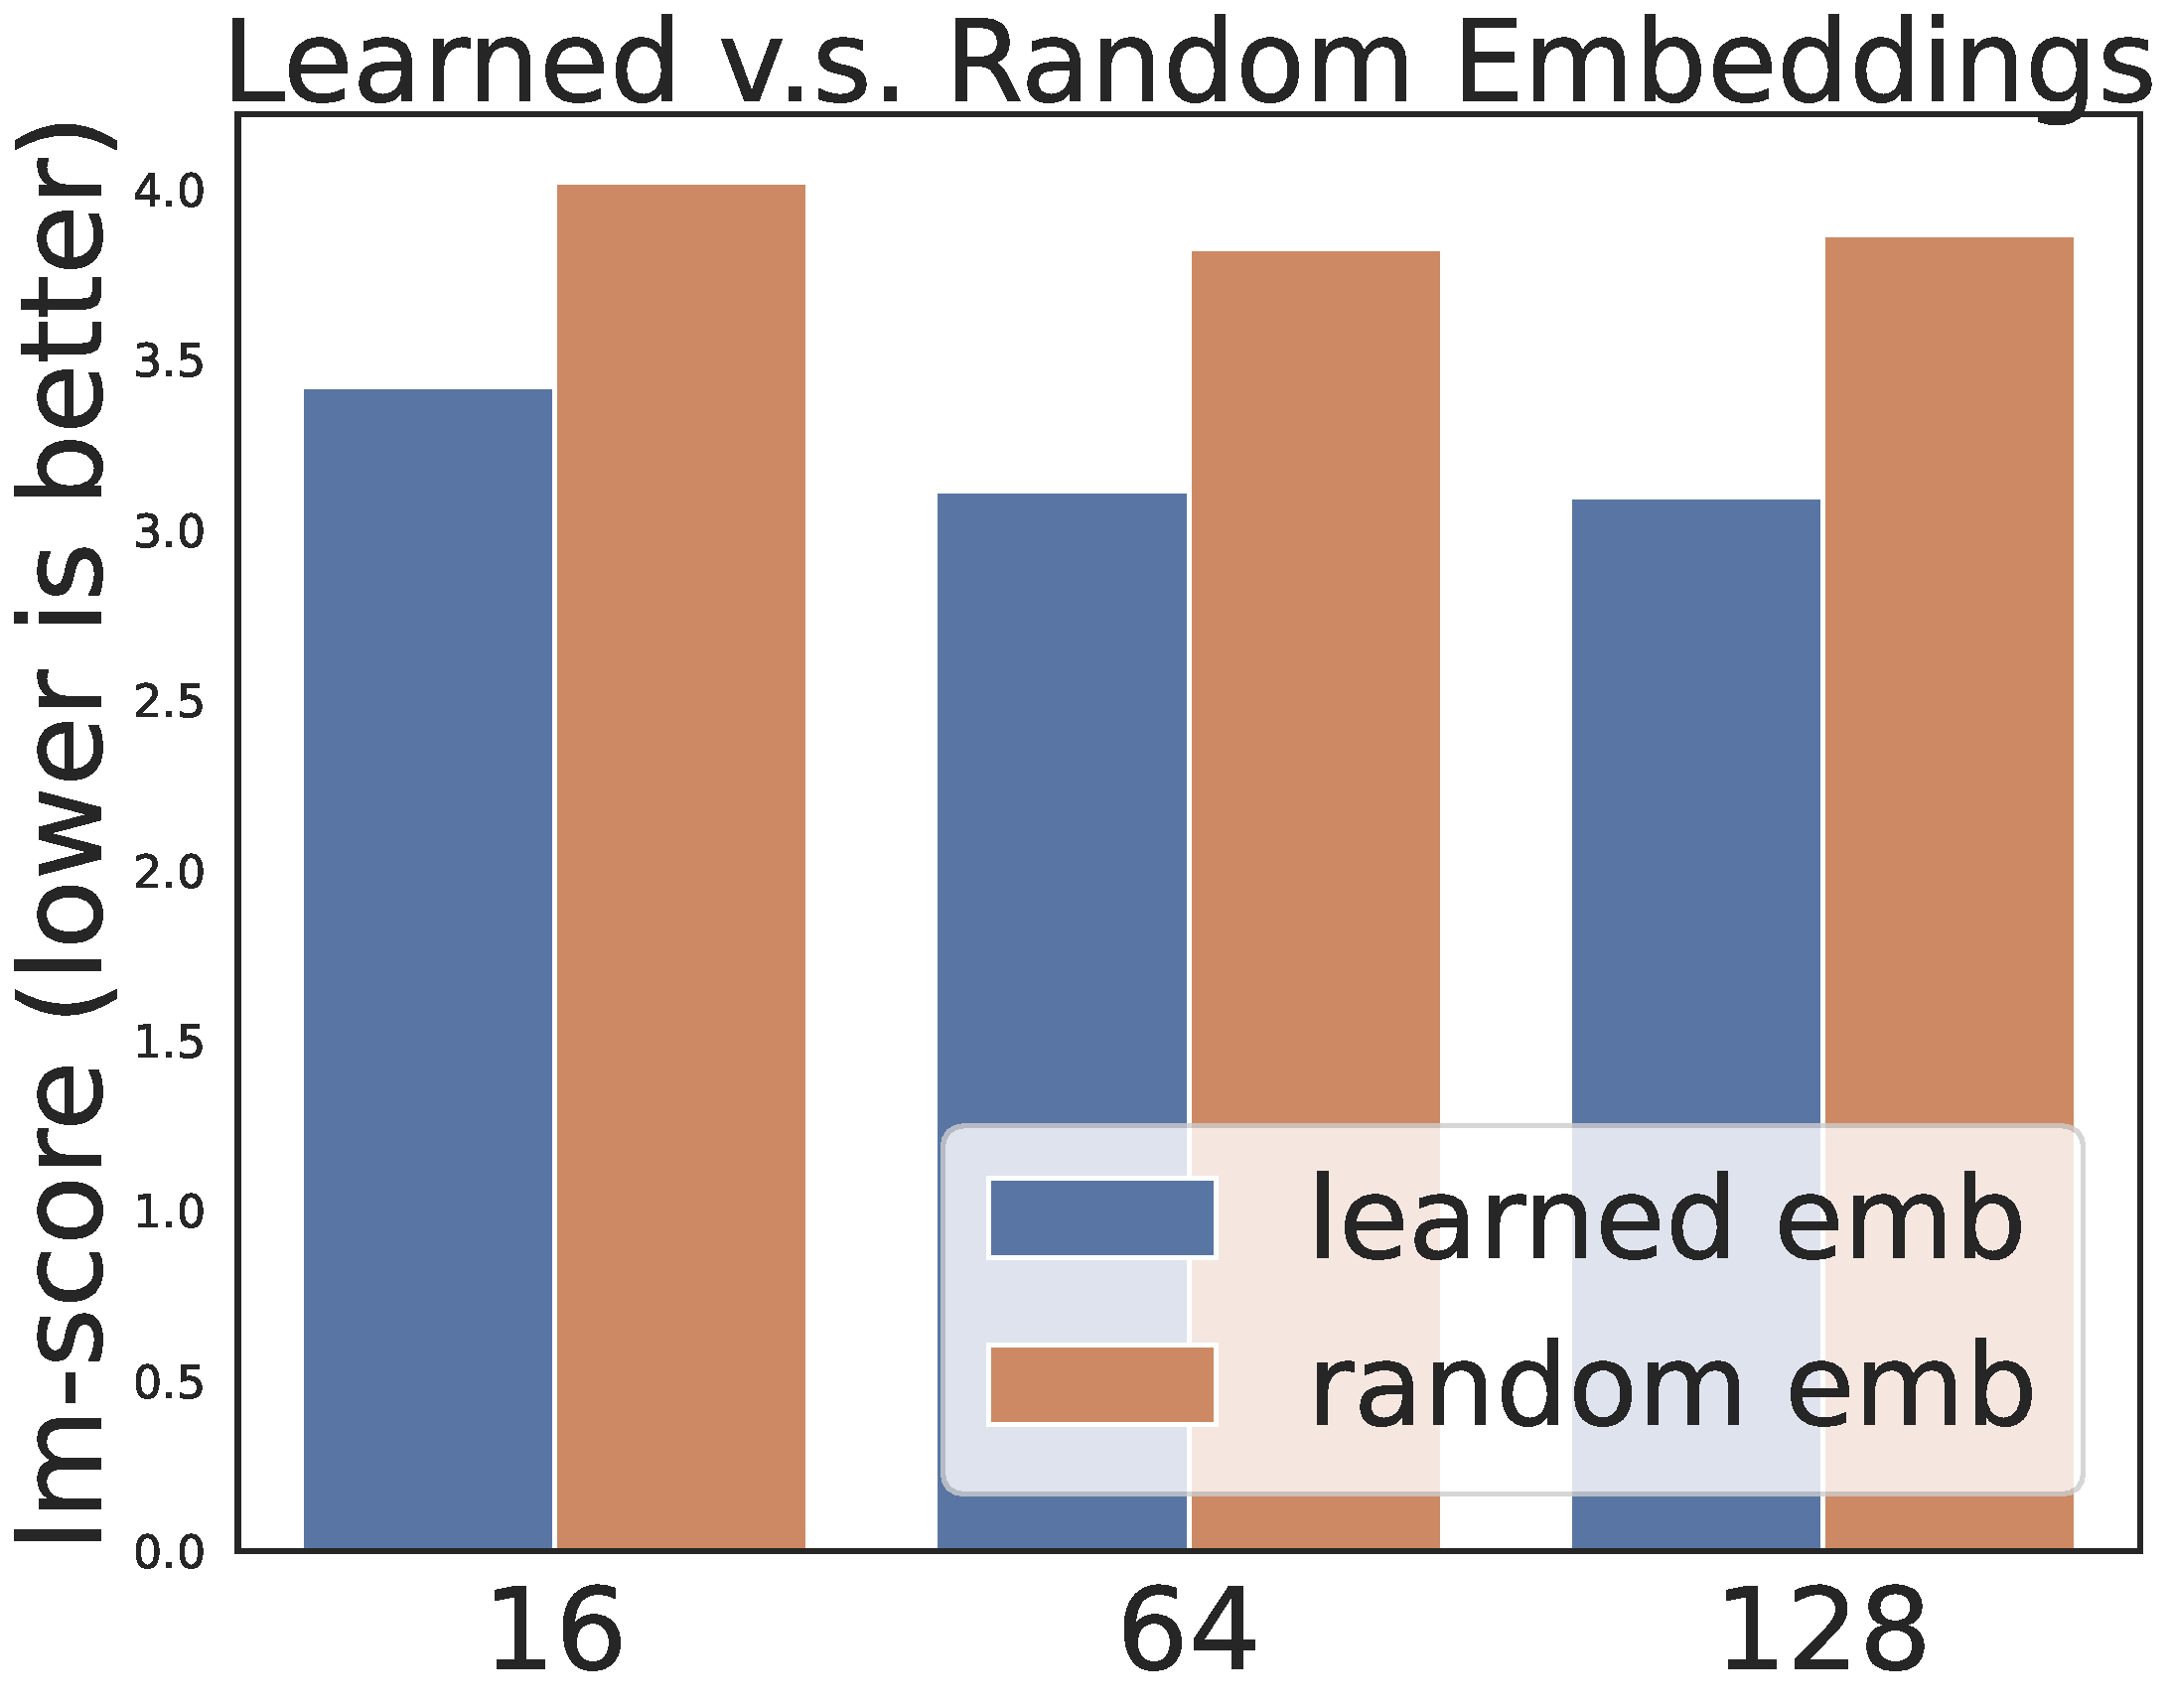
\includegraphics[width=0.25\textwidth]{fig/ablation_full1-2.pdf}
    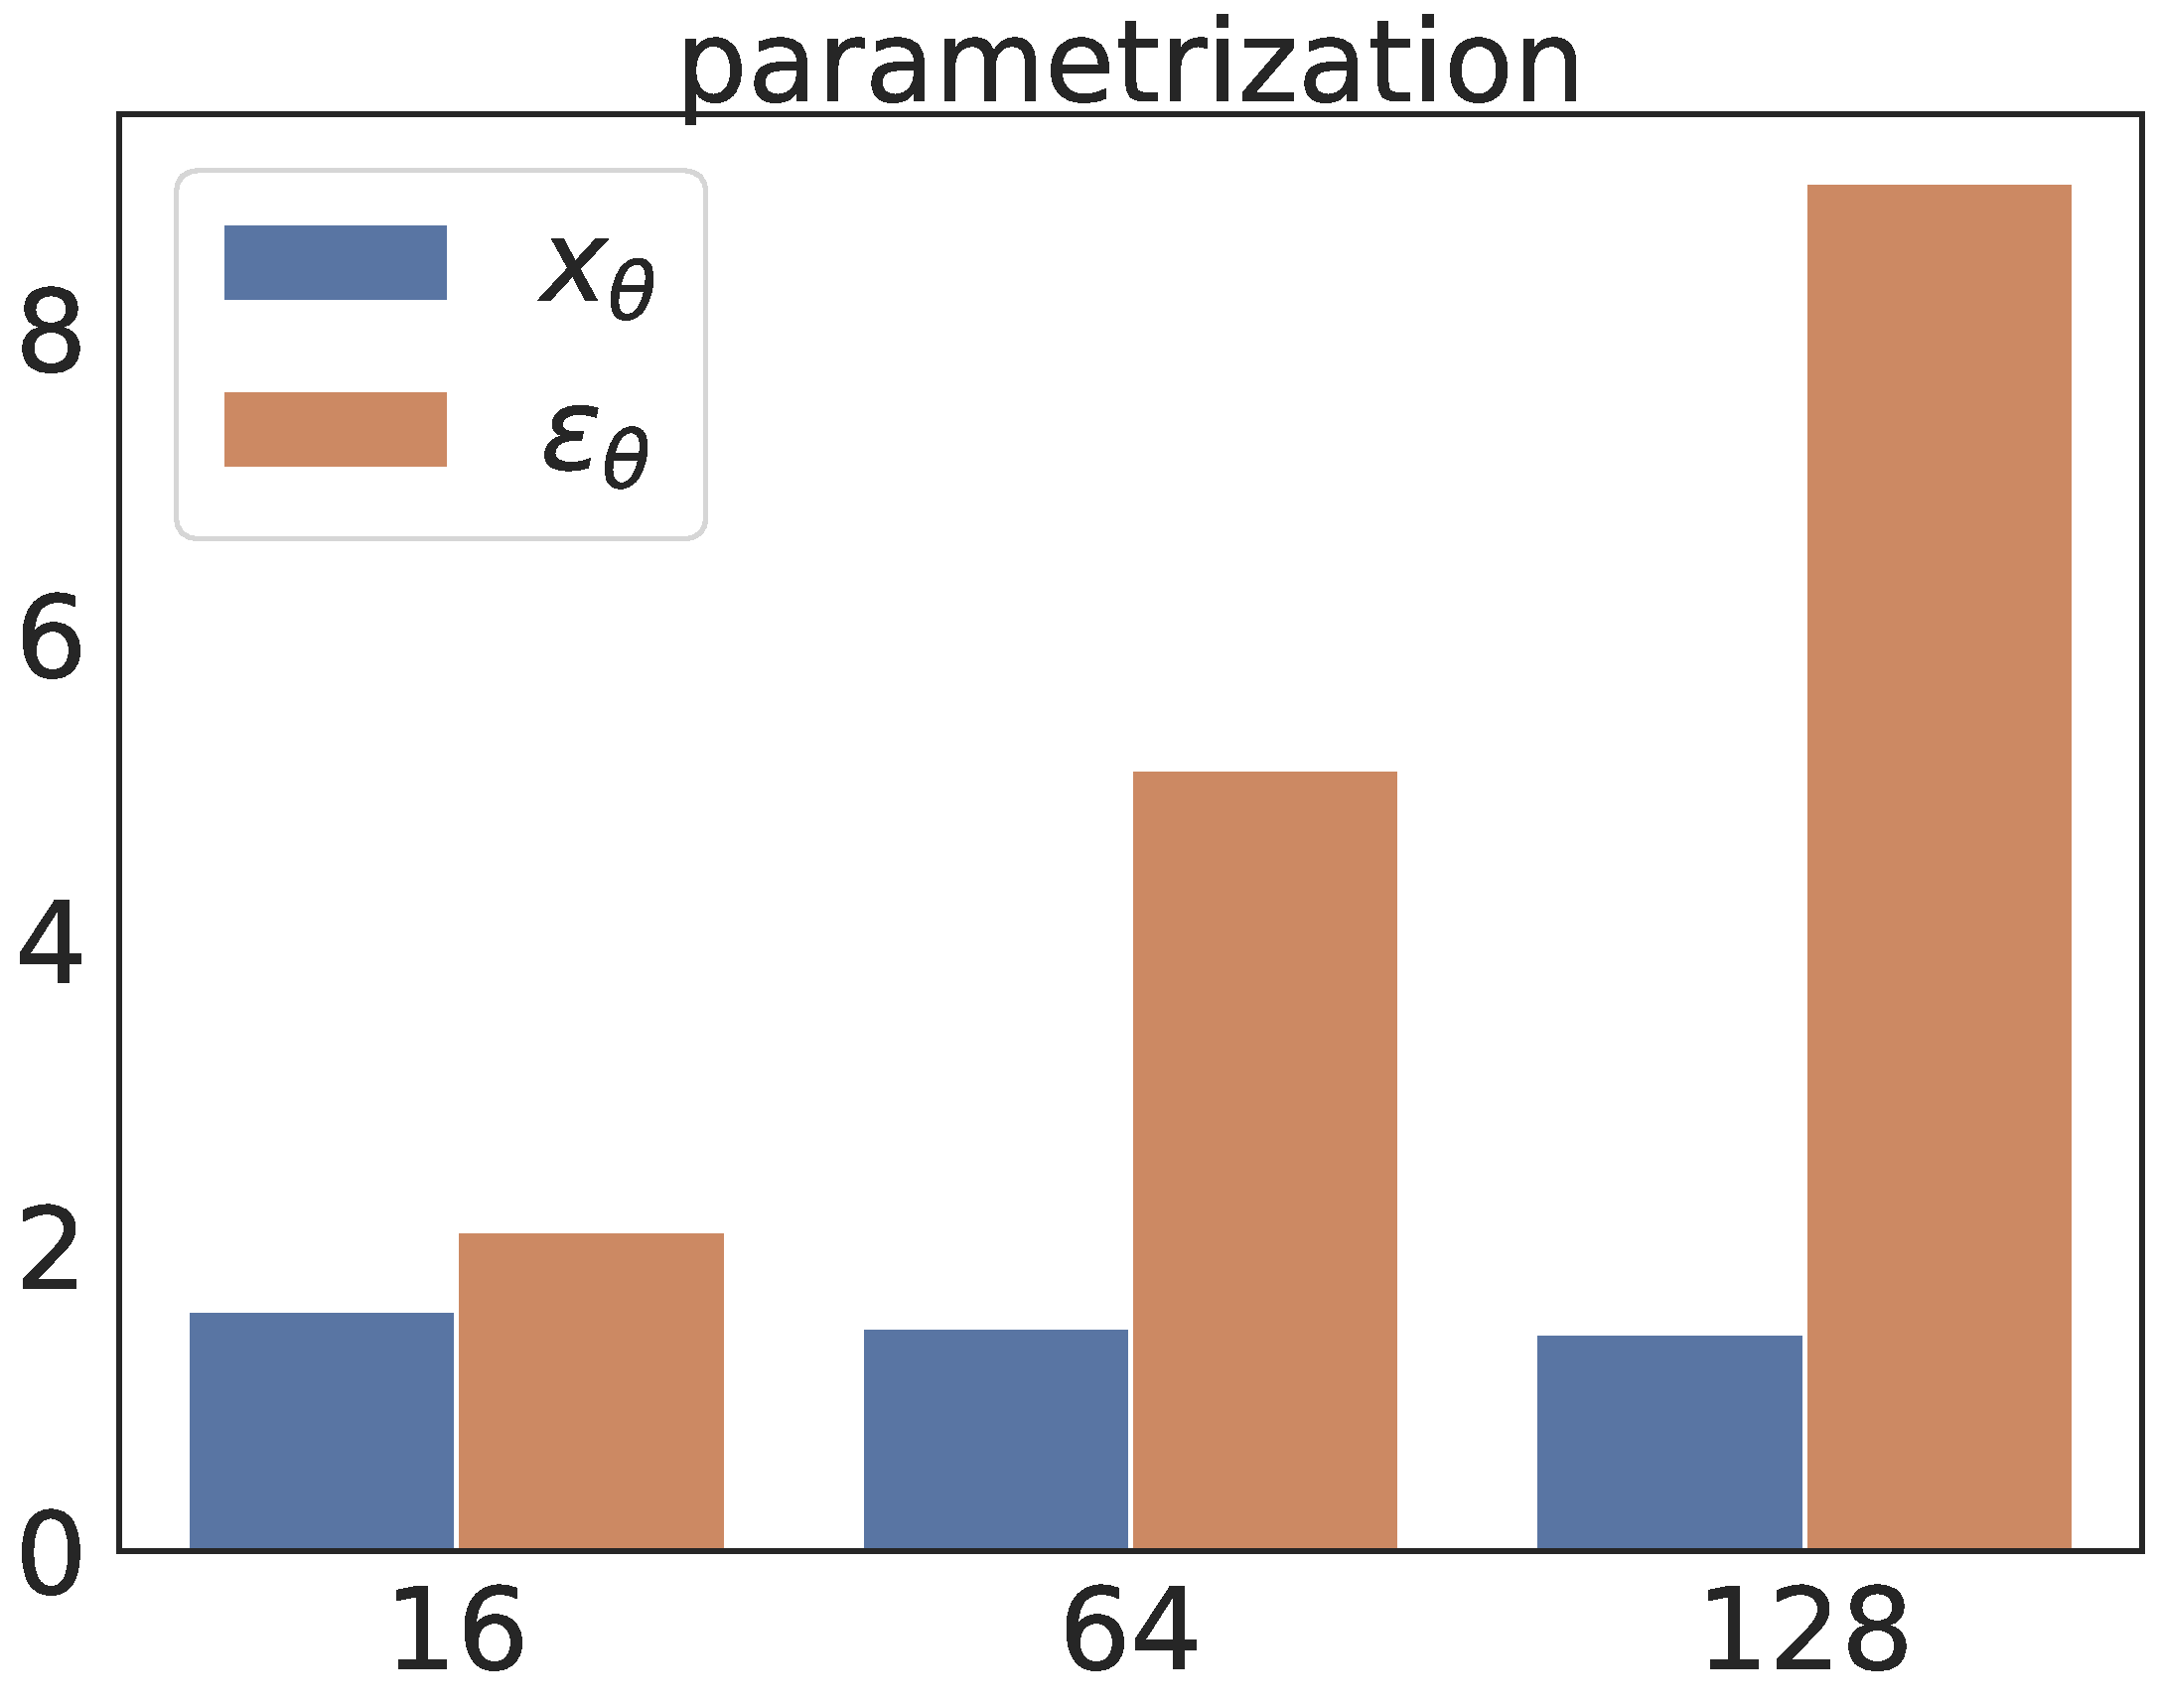
\includegraphics[width=0.25\textwidth]{fig/ablation_full2.pdf}
\caption{\label{fig:ablation}
我们通过 lm-score 衡量所提出设计选择的影响。我们发现，学到的 embeddings 和重参数化都显著提升了样本质量。
}
\end{wrapfigure}


我们通过两个消融研究验证 \cref{sec:method} 中所提出设计选择的重要性。我们在 500 个样本上使用 lm-score 衡量 Diffusion-LM 的样本质量~\cref{ssec:control_gen_setup}。

\textbf{学习式 vs. 随机 Embeddings（\cref{ssec:embeddings}）。}
学习式 embeddings 在 ROCStories 上优于随机 embeddings，而 ROCStories 是更难的语言建模任务。E2E 数据集上也有相同趋势，但幅度较小。


\textbf{目标参数化（\cref{ssec:rounding}）。}
我们提出让扩散模型直接预测 $\cx{0}$。这里，我们将其与图像生成中的标准参数化进行比较，后者通过噪声项 $\epsilon$ 参数化。\cref{fig:ablation}（右）显示，通过 $\cx{0}$ 参数化在不同维度上都能稳定取得良好性能，而通过 $\epsilon$ 参数化在小维度时表现尚可，但在较大维度时很快崩溃。




\section{结论与局限性}
我们提出 Diffusion-LM，这是一种基于连续扩散的新的可控语言模型，支持新的复杂细粒度控制任务形式。
我们展示了 Diffusion-LM 在 6 个细粒度控制任务上的成功：我们的方法几乎将先前方法的控制成功率翻倍，并且与需要额外训练的微调基线方法具有竞争力。

我们认为 Diffusion-LM 所支持的复杂控制很有吸引力，并且对 Diffusion-LM 显著偏离当前离散自回归生成范式这一点感到兴奋。与任何新技术一样，我们构建的 Diffusion-LM 也存在缺点：(1) 它具有更高的困惑度；(2) 解码明显更慢；%
以及 (3) 训练收敛更慢。我们相信，通过更多后续工作和优化，许多这些问题可以得到解决，而该方法将成为一种有吸引力的大规模可控生成方式。%



\begin{ack}
我们感谢 Yang Song、Jason Eisner、Tianyi Zhang、Rohan Taori、Xuechen Li、Niladri Chatterji 以及 p-lambda 小组成员在早期讨论和反馈中的帮助。我们衷心感谢 PECASE 奖项的支持。
Xiang Lisa Li 受 Stanford Graduate Fellowship 支持。
\end{ack}






\bibliography{anthology}



















\clearpage

 \appendix



\section{扩散噪声调度}
\newcommand{\sqrtt}{\textit{sqrt}\xspace} 
\newcommand{\cosine}{\textit{cosine}\xspace}
\newcommand{\linear}{\textit{linear}\xspace}

\label{app:noise}
\begin{wrapfigure}[11]{R}{0.25\textwidth}
\centering
\vspace{-10pt}
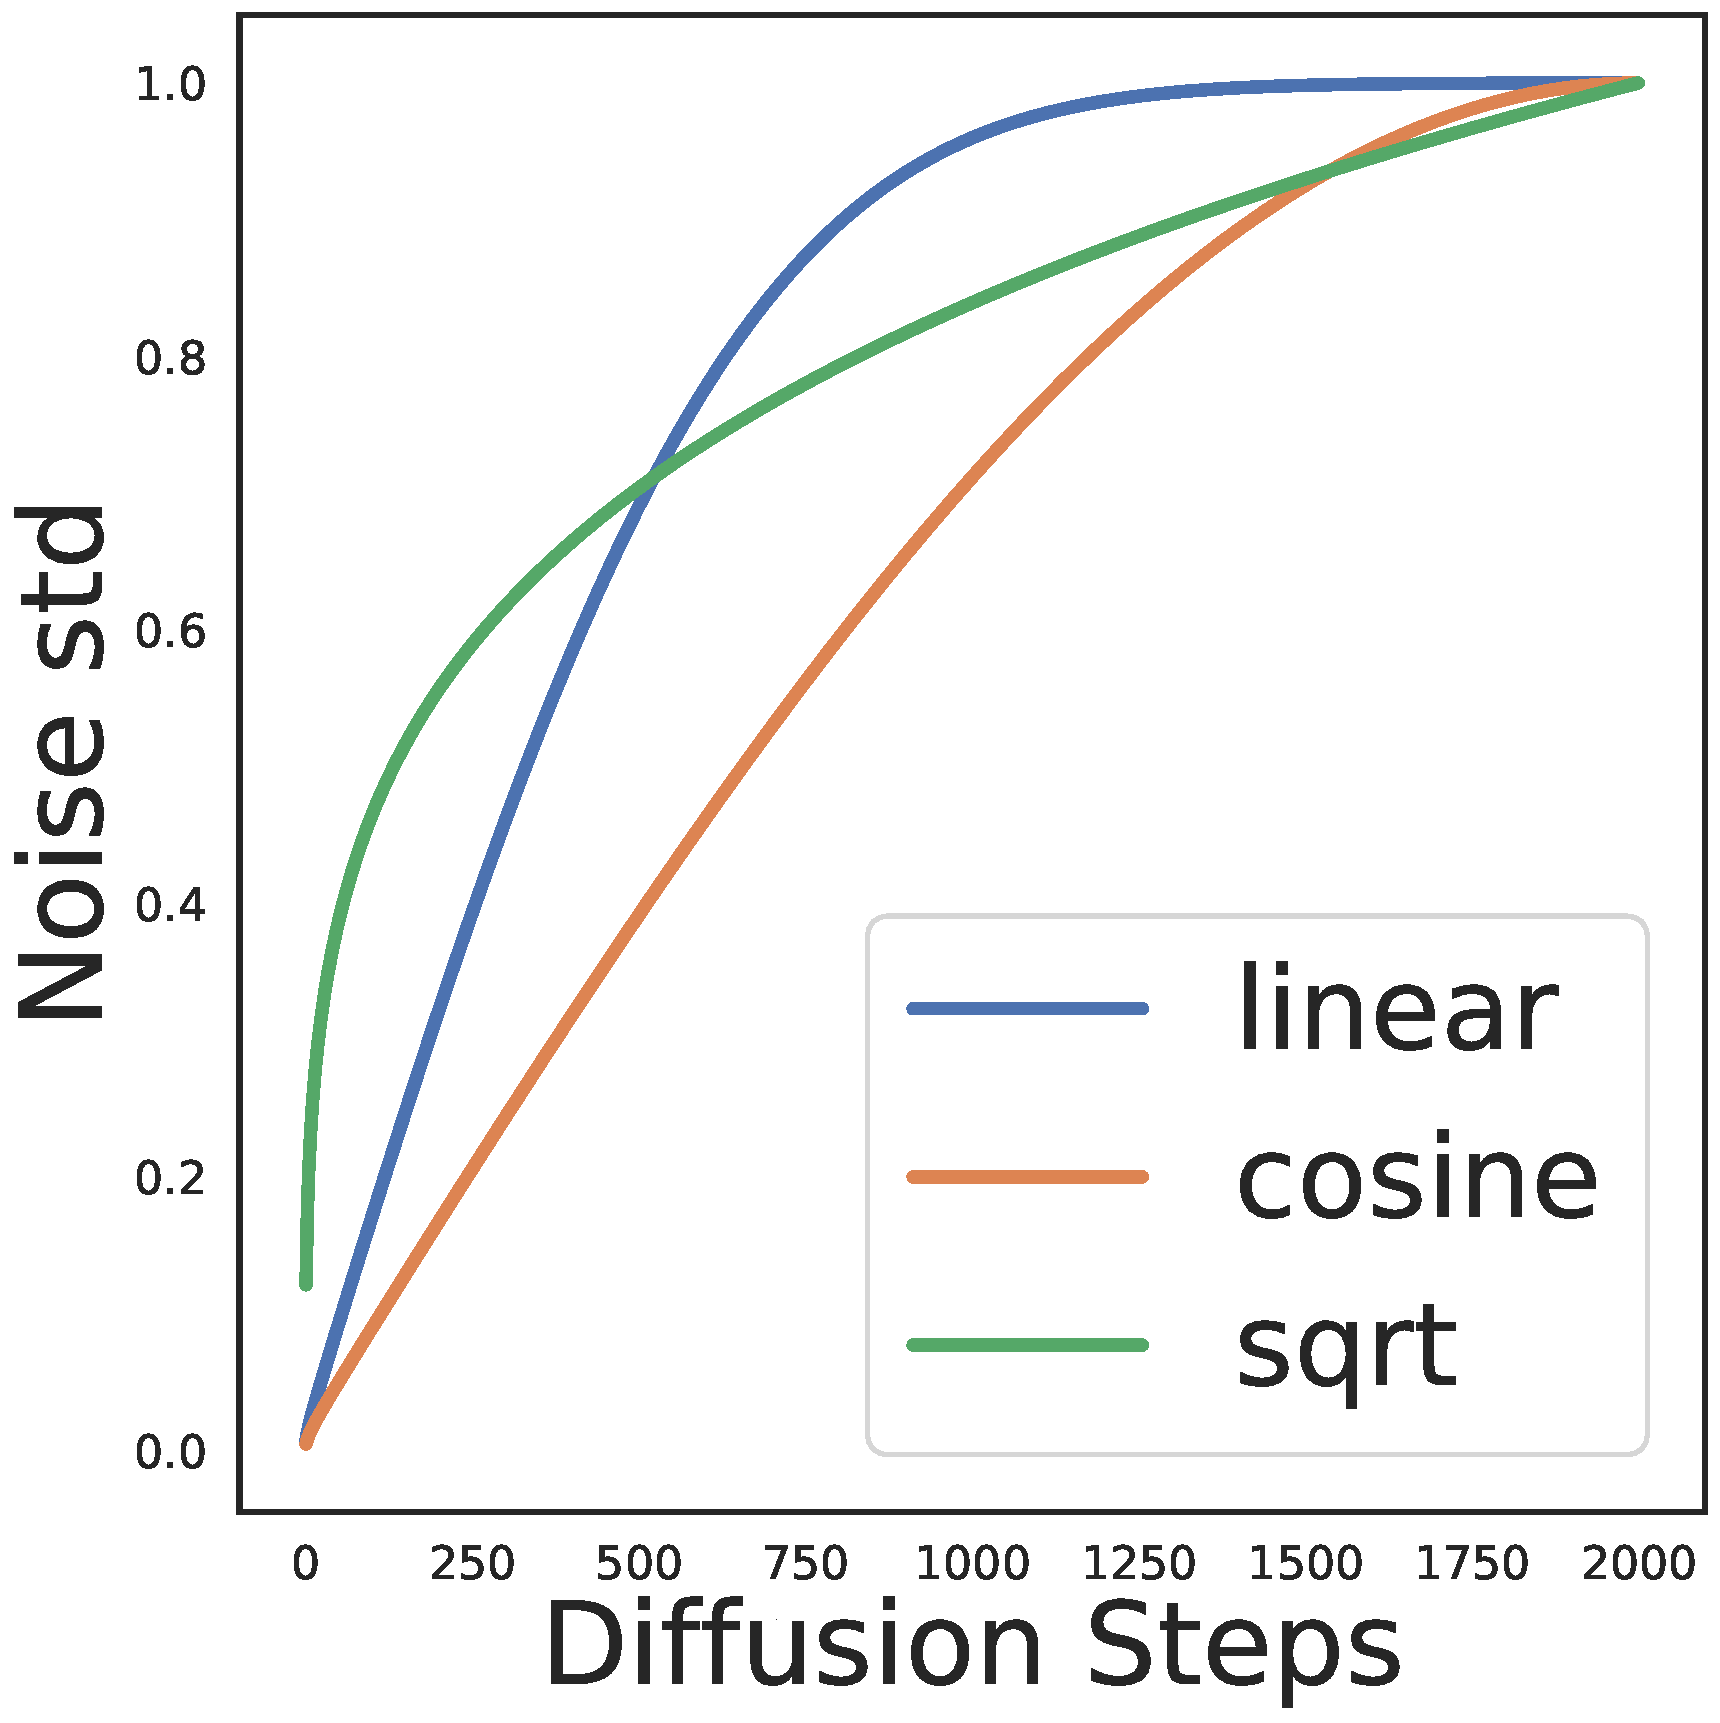
\includegraphics[width=0.9\linewidth]{fig/noise_schedule_v4.pdf}
\vspace{-3pt}
\caption{噪声调度 $\sqrt{1-\alphabar_t}$ 的可视化。\label{fig:noise}  }
\vspace{-10pt}
\end{wrapfigure}

由于扩散模型在所有扩散步骤上共享参数，噪声调度（由 $\alphabar_{1:T}$ 参数化）是一个重要超参数，它决定了我们为每个去噪问题分配多少权重。
我们发现，连续扩散的标准噪声调度对文本数据并不鲁棒。我们假设，文本的离散性质和 rounding 步骤使模型对 $t= 0$ 附近的噪声不敏感。具体而言，向词 embedding 添加少量 Gaussian 噪声不太可能改变其在 embedding 空间中的最近邻，因此 $t=0$ 附近的去噪任务较为容易。

为解决这一问题，我们引入一种更适合文本的新 \sqrtt 噪声调度，如 \cref{fig:noise} 所示，其定义为
$\alphabar_t = 1-\sqrt{t/T + s}$，其中 $s$ 是对应起始噪声水平的小常数\footnote{我们设 $s=$1e-4，$T=2000$，这使初始标准差为 $0.1$。}。与标准 \linear 和 \cosine 调度相比，我们的 \sqrtt 调度从更高噪声水平开始，并在前 50 步快速增加噪声。随后 \sqrtt 放慢注入噪声的速度，以避免在高噪声问题上花费太多步骤，因为这些问题可能过难而无法很好求解。





\section{超参数} 
\label{app:hyperparam} 
\paragraph{Diffusion-LM 超参数。}
Diffusion-LM 特有的超参数包括扩散步骤数、Diffusion-LM 的架构、embedding 维度和噪声调度。我们将扩散步骤设为 $2000$，架构设为 BERT-base \cite{Devlin2019BERTPO}，序列长度设为 $64$。
对于 embedding 维度，我们从 $d \in \{16, 64, 128, 256\}$ 中选择，并为 E2E 数据集选择 $d=16$，为 ROCStories 选择 $d=128$。
对于噪声调度，我们设计了 \sqrtt 调度（\cref{app:noise}），如 \cref{app:ablation} 所示，它对不同参数化和 embedding 维度更鲁棒。然而，一旦我们选择 $\cx{0}$-参数化（\cref{ssec:rounding}），\sqrtt 调度的优势就不那么显著。

\paragraph{训练超参数。}
我们使用 AdamW 优化器训练 Diffusion-LM，学习率从 1e-4 开始线性衰减，dropout 为 0.1，batch size 为 64；总训练迭代次数在 E2E 数据集上为 200K，在 ROCStories 数据集上为 800K。我们的 Diffusion-LM 在单个 GPU 上训练：NVIDIA RTX A5000、NVIDIA GeForce RTX 3090 或 NVIDIA A100。在单个 A100 GPU 上训练 200K 次迭代约需 5 小时。

为稳定 $\Lvlb^{\text{e2e}}$ 目标下的训练，我们发现需要将梯度裁剪设为 1.0，并应用重要性采样对 $\Lvlb$ 中的每一项重新加权 \cite{nichol2021improved}。对于 $\Lsimple^{\text{e2e}}$ 目标，这两个技巧都不是必需的。

\paragraph{可控生成超参数。} 为实现可控生成，我们在 Diffusion-LM 的连续隐变量上执行梯度更新。
我们使用 AdaGrad 优化器 \cite{Duchi2010AdaptiveSM} 更新隐变量，并调节学习率 $\text{lr} \in \{0.05, 0.1, 0.15, 0.2\}$ 和权衡参数 $\lambda \in \{0.1, 0.01, 0.001, 0.0005\}$。不同 plug-and-play 可控生成方法通过调节不同超参数来权衡流畅性与控制：PPLM 使用每个 token 的梯度更新次数，记为 $k$，我们调节 $k \in \{10, 30\}$。FUDGE 使用权衡参数 $\lambda_{\text{FUDGE}}$，我们调节 $\lambda_{\text{FUDGE}} \in \{16, 8, 4, 2 \}$。\cref{tab:hyper} 包含每个控制任务所选的全部超参数。PPLM 和 FUDGE 都有额外超参数，我们遵循原论文的说明进行设置。对于 PPLM，我们将学习率设为 0.04，将 KL-scale 设为 0.01。对于 FUDGE，我们将 precondition top-K 设为 200，将 post top-K 设为 10。

\newcommand{\tradeoff}{tradeoff}
\begin{table*}
\centering
\resizebox{0.9\columnwidth}{!}{
\begin{tabular}{lcc|cc|cc|cc|cc}
\toprule
          & \multicolumn{2}{c|}{Semantic} & \multicolumn{2}{c|}{Parts-of-speech} & \multicolumn{2}{c|}{Syntax Tree} & \multicolumn{2}{c|}{Syntax Spans} & \multicolumn{2}{c}{Length}  \\
& \tradeoff        & lr       & \tradeoff     & lr    & \tradeoff     & lr     & \tradeoff     & lr    &  \tradeoff     & lr    \\ \hline
PPLM      &  30  & 0.04  &  - & - & - & - & - & - & - &  - \\
FUDGE     & 8.0  & -  &20.0 & - & 20.0 & - & 20.0 & - & 2.0 & -  \\
Diffusion-LM & 0.01 & 0.1 & 0.0005 & 0.05 & 0.0005 & 0.2 &  0.1 & 0.15 & 0.01 & 0.1 \\
\bottomrule
\end{tabular}
}
\caption{\label{tab:hyper} 可控生成方法的超参数。}
\end{table*}

\section{解码速度}
从 Diffusion-LM 采样需要迭代 2000 个扩散步骤，产生 $O(2000)$ 次 $\xxtheta$ 模型调用。相比之下，从自回归 LM 采样需要 $O(n)$，其中 $n$ 是序列长度。因此，在短序列和中等长度序列场景中，解码 Diffusion-LM 比解码自回归 LM 更慢。具体而言，解码 50 个长度为 64 的序列大约需要 1 分钟。

为加速解码，我们尝试在生成扩散过程中跳过步骤，将 2000 步下采样到 200 步。具体而言，我们设 $T=200$ 并下采样噪声调度 $\alphabar_{t} = \alphabar_{10t}$，这等价于将每个单位转移设为转移 $\cx{t} \rightarrow \cx{t+10}$。我们使用这一新的噪声调度和离散化来解码 Diffusion-LM。我们发现，这种简单的做法不会损害 E2E 等简单语言建模任务的样本质量，但会损害 ROCStories 等更难语言建模任务的样本质量。

对于 plug-and-play 可控生成任务，现有方法甚至更慢。
PPLM 生成 50 个样本大约需要 80 分钟（不使用 batching），因为它需要对每个 token 执行 30 次梯度更新。
FUDGE 生成 50 个样本需要 50 秒（使用 batching），因为它需要为每个部分序列调用轻量分类器，每个 token 需要 200 次分类器调用，产生 $100 \times$ 序列长度次调用。我们可以批处理分类器调用，但由于 GPU 内存有限，这有时会限制跨样本 batching。
我们的 Diffusion-LM 生成 50 个样本大约需要 80 秒（使用 batching）。我们的方法将扩散步骤数下采样到 200，并且每个扩散步骤需要 3 次分类器调用，总共 600 次模型调用。

\section{分类器引导控制的分类器}
\textbf{Semantic Content.} 我们训练一个自回归 LM（GPT-2 small 架构），在文本条件下预测 (field, value) 对。为参数化 $\log p(\cc \mid \cx{t})$，我们计算每个 token 上 ``value'' 的 logprob。


\textbf{Parts-of-speech.} 该分类器由 parts-of-speech 标注器参数化，它估计在隐变量条件下目标 POS 序列的概率。该标注器使用 BERT-base 架构：输入是拼接的词 embedding，输出是每个输入词在所有 POS 标签上的 softmax 分布。$\log p(\cc \mid  \cx{t})$ 是序列中每个词的 POS log-probs 之和。

\textbf{Syntax Tree.} 我们训练一个基于 Transformer 的 constituency parser \cite{kitaev-klein-2018-constituency}。我们的解析器对每个 span 作局部归一化预测，预测 ``not a constituent'' 或该成分的标签（例如 Noun Phrase）。
$\log p(\cc \mid  \cx{t})$ 是序列中每个带标签 span 和非成分 span 的 log-probs 之和。


\textbf{Syntax Span.} 我们使用为 syntax tree 训练的同一解析器。$\log p(\cc \mid  \cx{t})$ 是目标 span 被标注为目标标签的 log-probability。

\section{端到端目标推导}
\label{app:derive}
对于连续扩散模型（\cref{ssec:diffusion_setup}），$\Lsimple$ 通过对典型目标 $\Lvlb$ 的每一项重新加权而推导得到。
$\Lvlb$ 中的前 $T$ 项都是两个 Gaussian 分布之间的 KL divergence，具有闭式解。以第 $t$ 项为例：
\begin{equation}
\mathop{\mathbb{E}}_{q(\cx{1:T} | \cx{0})} \left[ \log \frac{q(\cx{t-1} | \cx{0},\cx{t})} {\ptheta(\cx{t-1} | \cx{t}) }\right] = \mathop{\mathbb{E}}_{ q(\cx{1:T} | \cx{0})}  \left[ \frac{1}{2\sigma_t^2}  || \mu_\theta(\cx{t}, t) - \hat{\mu}(\cx{t}, \cx{0}) ||^2\right] + C, 
\label{app:eqn:simple}
\end{equation}
其中 $C$ 是常数，$\hat{\mu}$ 是后验 $q(\cx{t-1} | \cx{0},\cx{t})$ 的均值，$\mu_\theta$ 是扩散模型预测的 $\ptheta(\cx{t-1} \mid \cx{t})$ 的均值。直观上，这一简化将 $\cx{t-1}$ 的预测均值与其真实后验均值匹配。该简化移除了常数 $C$ 和缩放因子 $\frac{1}{2\sigma_t^2}$，得到 $\Lsimple$ 中的一项：$\mathop{\mathbb{E}}_{ q(\cx{1:T} | \cx{0})}  \left[  || \mu_\theta(\cx{t}, t) - \hat{\mu}(\cx{t}, \cx{0}) ||^2\right]$。

为应用连续扩散来建模离散文本，我们设计 Diffusion-LM（\cref{ssec:embeddings}），并提出新的端到端训练目标（\cref{obj:e2e}），以联合学习扩散模型和 embedding 参数。$\Lvlb^{\text{e2e}}$ 可写为
\begin{align*}
    \mathcal{L}^\text{e2e}_{\text{vlb}} (\ww) &= \mathop{\mathbb{E}}_{q_\phi(\cx{0} | \ww)}\left[\mathcal{L}_{\text{vlb}} (\cx{0}) + \log \qphi(\cx{0} | \ww) - \log \ptheta(\ww | \cx{0})]\right] \\
    &= \mathop{\mathbb{E}}_{q_\phi(\cx{0:T} | \ww)}  \left[\underbrace{\log \frac{q(\cx{T} | \cx{0})}{\ptheta(\cx{T})}}_{L_T} + \sum_{t=2}^T \underbrace{\log \frac{q(\cx{t-1} | \cx{0},\cx{t})} {\ptheta(\cx{t-1} | \cx{t}) }}_{L_{t-1}} - \underbrace{\frac{\log \qphi(\cx{0} | \ww)}{\log \ptheta( \cx{0} | \cx{1})}}_{L_{0}}     - \underbrace{\log \ptheta(\ww | \cx{0})}_{L_\text{round}}\right]  \\
\end{align*}
我们应用将 $\Lvlb \rightarrow \Lsimple$ 的同一简化，将 $\mathcal{L}^\text{e2e}_{\text{vlb}} \rightarrow \Lsimpleee$：
\begin{align*}
    \mathop{\mathbb{E}}_{q_\phi(\cx{0:T} | \ww)} [L_T] & \rightarrow \mathbb{E}[||\mathop{\mathbb{E}}_{\cx{T}\sim q}[\cx{T}| \cx{0}] - 0 ||^2] = \mathbb{E}[||\hat{\mu}(\cx{T}; \cx{0})] ||^2] \\
    \mathop{\mathbb{E}}_{q_\phi(\cx{0:T} | \ww)} [L_{t-1}] & \rightarrow \mathbb{E}[|| \mathop{\mathbb{E}}_{\cx{t-1}\sim q}[\cx{t-1}| \cx{0}, \cx{t}] - \mathop{\mathbb{E}}_{\cx{t-1} \sim \ptheta}  [\cx{t-1} | \cx{t}] ||^2] =\mathbb{E}[ ||\hat{\mu}(\cx{t}, \cx{0})-\mu_\theta(\cx{t}, t) ||^2]\\
    \mathop{\mathbb{E}}_{q_\phi(\cx{0:T} | \ww)} [L_{0}] & \rightarrow \mathbb{E}[|| \mathop{\mathbb{E}}_{\cx{0}\sim\qphi} [\cx{0} \mid \ww] - \mathop{\mathbb{E}}_{\cx{0} \sim \ptheta} [\cx{0}  \mid \cx{1} ] ||^2] = \mathbb{E}[ ||\Emb(w)-\mu_\theta(\cx{1}, 1) ||^2]
\end{align*}

值得注意的是，如果噪声调度满足 $\alphabar_T = 0$，从而保证 $\cx{T}$ 是纯 Gaussian 噪声，则第一项是常数。
相反，如果噪声调度没有一直进行到使 $\cx{T}$ 成为纯 Gaussian 噪声，我们需要包含该正则项，以防止 embedding 学到过大的范数。具有大范数的 embedding 是一种退化解，因为即便它使所有其他去噪转移都容易预测，也不可能准确地从 $p(\cx{T})$ 采样。

组合这些项得到 $\Lsimpleee$。
\begin{align*}
    \mathcal{L}^\text{e2e}_\text{simple} (\ww) & =  \mathop{\mathbb{E}}_{\qphi(\cx{0:T} | \ww)}  \left[||\hat{\mu}(\cx{T}; \cx{0})||^2 + \sum_{t=2}^T [||\hat{\mu}(\cx{t}, \cx{0})-\mu_\theta(\cx{t}, t) ||^2] \right] \\
& ~~~~~~~~~~~ + \mathop{\mathbb{E}}_{\qphi(\cx{0:1} | \ww)} \left[|| \Emb(\ww) - \mu_\theta(\cx{1}, 1) ||^2  - \log \ptheta(\ww | \cx{0})\right].
\end{align*}

直观上，我们学习一个 Transformer 模型，它以 $(\cx{t}, t) \in (\mathbb{R}^{nd}, \mathbb{R})$ 为输入，目标是预测 $\cx{t-1} \in \mathbb{R}^{nd}$ 的分布。值得注意的是，该 Transformer 模型在所有扩散步骤 $t = 1\dots T$ 上共享。如我们在 $\Lsimpleee$ 推导中所示，最自然的做法是直接参数化神经网络以预测 $\cx{t-1} \mid \cx{t}$ 的均值，我们称之为 $\mu_\theta$-参数化。

还存在其他参数化，它们与 $\mu_\theta$-参数化仅相差一个缩放常数。例如在 \cref{ssec:rounding} 中，我们可以训练 Transformer 模型通过 $\xxtheta(\cx{t}, t)$ 直接预测 $\cx{0}$，并使用易处理的 Gaussian 后验 $q(\cx{t-1} \mid \cx{0}, \cx{t})$ 计算 $\cx{t-1}$ 的均值；在预测的 $\cx{0}$ 和观测到的 $\cx{t}$ 条件下，该均值具有闭式解：$ \frac{\sqrt{\alphabar_{t-1}} \beta_t}{1-\alphabar_t}\cx{0} + \frac{\sqrt{\alpha_t} (1-\alphabar_{t-1})}{1-\alphabar_t} \cx{t}$。
\begin{align*}
& ||\hat{\mu}(\cx{t}, \cx{0})-\mu_\theta(\cx{t}, t) ||^2 \\
= &  ||(\frac{\sqrt{\alphabar_{t-1}} \beta_t}{1-\alphabar_t}\cx{0} + \frac{\sqrt{\alpha_t} (1-\alphabar_{t-1})}{1-\alphabar_t} \cx{t}) - (\frac{\sqrt{\alphabar_{t-1}} \beta_t}{1-\alphabar_t}\xxtheta(\cx{t}, t) + \frac{\sqrt{\alpha_t} (1-\alphabar_{t-1})}{1-\alphabar_t} \cx{t})||^2\\
= & ||\frac{\sqrt{\alphabar_{t-1}} \beta_t}{1-\alphabar_t}(\cx{0} - \xxtheta(\cx{t}, t))||^2\\
\propto &  ||\cx{0} - \xxtheta(\cx{t}, t)||^2
\end{align*}
这两种参数化仅相差常数缩放，并且如 \cref{ssec:rounding} 所讨论，为减少 rounding 错误，我们将 $\cx{0}$-参数化应用于 $\Lsimpleee$ 中的所有项：
\begin{align*}
    \mathcal{L}^\text{e2e}_{\cx{0}\text{-simple}} (\ww) & =  \mathop{\mathbb{E}}_{\qphi(\cx{0:T} | \ww)}  \left[||\hat{\mu}(\cx{T}; \cx{0})||^2 + \sum_{t=2}^T [||\cx{0}-\xxtheta(\cx{t}, t) ||^2] \right] \\
& ~~~~~~~~~~~ + \mathop{\mathbb{E}}_{\qphi(\cx{0:1} | \ww)} \left[|| \Emb(\ww) - \xxtheta(\cx{1}, 1) ||^2  - \log \ptheta(\ww | \cx{0})\right].
\end{align*}

为从具有 $\cx{0}$-参数化的 Diffusion-LM 生成样本，在每个扩散步骤，模型通过 $\xxtheta (\cx{t}, t)$ 估计 $\cx{0}$，随后我们从 $q(\cx{t-1} \mid \xxtheta (\cx{t}, t), \cx{t})$ 采样 $\cx{t-1}$，并将其作为下一扩散步骤的输入。






\section{对数似然模型与结果}
\label{app:simplex}

为研究 Diffusion-LM 的对数似然性能，我们对 \cref{sec:method} 的训练过程做出若干改变。
最终，本节描述的对数似然改进在我们的实验中没有转化为更好的生成质量，因此本文其余部分聚焦于原始方法。
我们的似然模型训练如下：
\begin{itemize}
    \item 我们不是在低维 token embeddings 序列上训练扩散模型，而是直接在 one-hot token 向量序列上训练模型。
    \item 遵循 \citet{kingma2021variational} 的设置，我们针对对数似然界训练连续时间扩散模型，并与模型其余部分同时学习噪声调度，以最小化损失方差。
    \item 由于我们的模型预测 one-hot 向量序列，我们在其输出处使用 softmax 非线性，并将损失函数中的所有平方误差项替换为 cross-entropy 项。尽管我们仍用带平方误差项的原始损失进行评估，但这种替代损失选择带来了更好的优化。
    \item 在任何 Transformer 层之前，模型对输入应用如下变换：$x := \mathrm{softmax}(\alpha(t) x + \beta(t))$，其中 $\alpha(t) \in \mathbb{R}$ 和 $\beta(t) \in \mathbb{R}^v$ 是由 MLP 参数化的扩散时间步 $t$ 的学习函数（$v$ 是词表大小）。
    \item 在推理时，我们省略 \cref{ssec:rounding} 中的 rounding 过程。
\end{itemize}
关于精确的模型架构和训练超参数细节，请参见我们发布的代码。

我们在 E2E 和 ROCStories 上训练这些扩散模型以及基线自回归 Transformers，并在 \cref{tab:ppl} 中报告对数似然。
我们训练两种规模的 Transformers：约 100M 参数的 ``small'' 模型和约 300M 参数的 ``medium'' 模型。
E2E 和 ROCstories 都是足够小的数据集，因此我们的所有模型都在训练早期达到最小测试损失（随后过拟合）。
为进一步比较大数据集场景下的模型性能，我们还给出 ``ROCStories (+GPT-J)'' 实验：通过在原始 ROCStories 数据上微调 GPT-J \citep{gpt-j}，生成 8M 个合成 ROCStories 训练数据示例，先在合成数据集上预训练模型，然后在原始 ROCStories 数据上微调并评估。

\begin{table*}
    \centering
\begin{tabular}{lcc|cc|cc|cc|cc}
\toprule
    Dataset                & Small AR    & Small Diffusion     & Medium Diffusion\\
    E2E                    & 1.77    & 2.28 & -\\
    ROCStories             & 3.05    & 3.88 & -\\
    ROCStories (+GPT-J)    & 2.41    & 3.59 & 3.10\\

\bottomrule
\end{tabular}
\caption{\label{tab:ppl} 对数似然结果（nats per token）}
\end{table*}

\section{定性示例}
\label{app:qualitative}

我们展示 Diffusion-LM 在无条件生成和 $5$ 个控制任务上的随机采样输出。\cref{app:qualitative-unc} 展示无条件生成结果。
\cref{app:qualitative-span}, \cref{app:qualitative-pos}, \cref{app:qualitative-content} 和 \cref{app:qualitative-syntax} 分别展示 span 控制、POS 控制、语义内容控制和 syntax tree 控制的定性样本。
\cref{app:qualitative-length} 展示长度控制结果。


\section{附加消融研究}
\label{app:ablation}
除了 \cref{sec:ablation} 中的 2 个消融研究外，我们在 \cref{app:tab:ablation} 中提供关于架构选择和噪声调度的更多消融结果。

\textbf{学习式 vs. 随机 Embeddings（\cref{ssec:embeddings}）。}
如 \cref{app:tab:ablation} 第一行所示，学习式 embeddings 在 ROCStories 和 E2E 数据集上分别比随机 embeddings 高 xx percent 和 xx percent。


\textbf{噪声调度（\cref{app:noise}）。}
我们将 \sqrtt 调度与为图像建模提出的 \cosine \cite{nichol2021improved} 和 \linear \cite{ho2020denoising} 调度进行比较。\cref{app:tab:ablation} 中间一行表明，\sqrtt 调度在所有维度和参数化选择上都取得一致良好且稳定的性能。虽然在 $\cx{0}$-参数化下 \sqrtt 调度不那么重要，但我们看到它在 $\epsilon$ 等替代参数化下提供了显著更鲁棒的噪声调度。

\paragraph{Transformer vs. U-Net。}
\citet{ho2020denoising} 中的 U-Net 架构使用 2D-convolutional layers，我们模仿所有模型架构，但将 2D-conv 改为适合文本数据的 1D-conv。
\cref{app:tab:ablation}（最后一行）显示 Transformer 架构优于 U-Net。

\begin{figure}

 \vspace{-10pt}
    \centering
    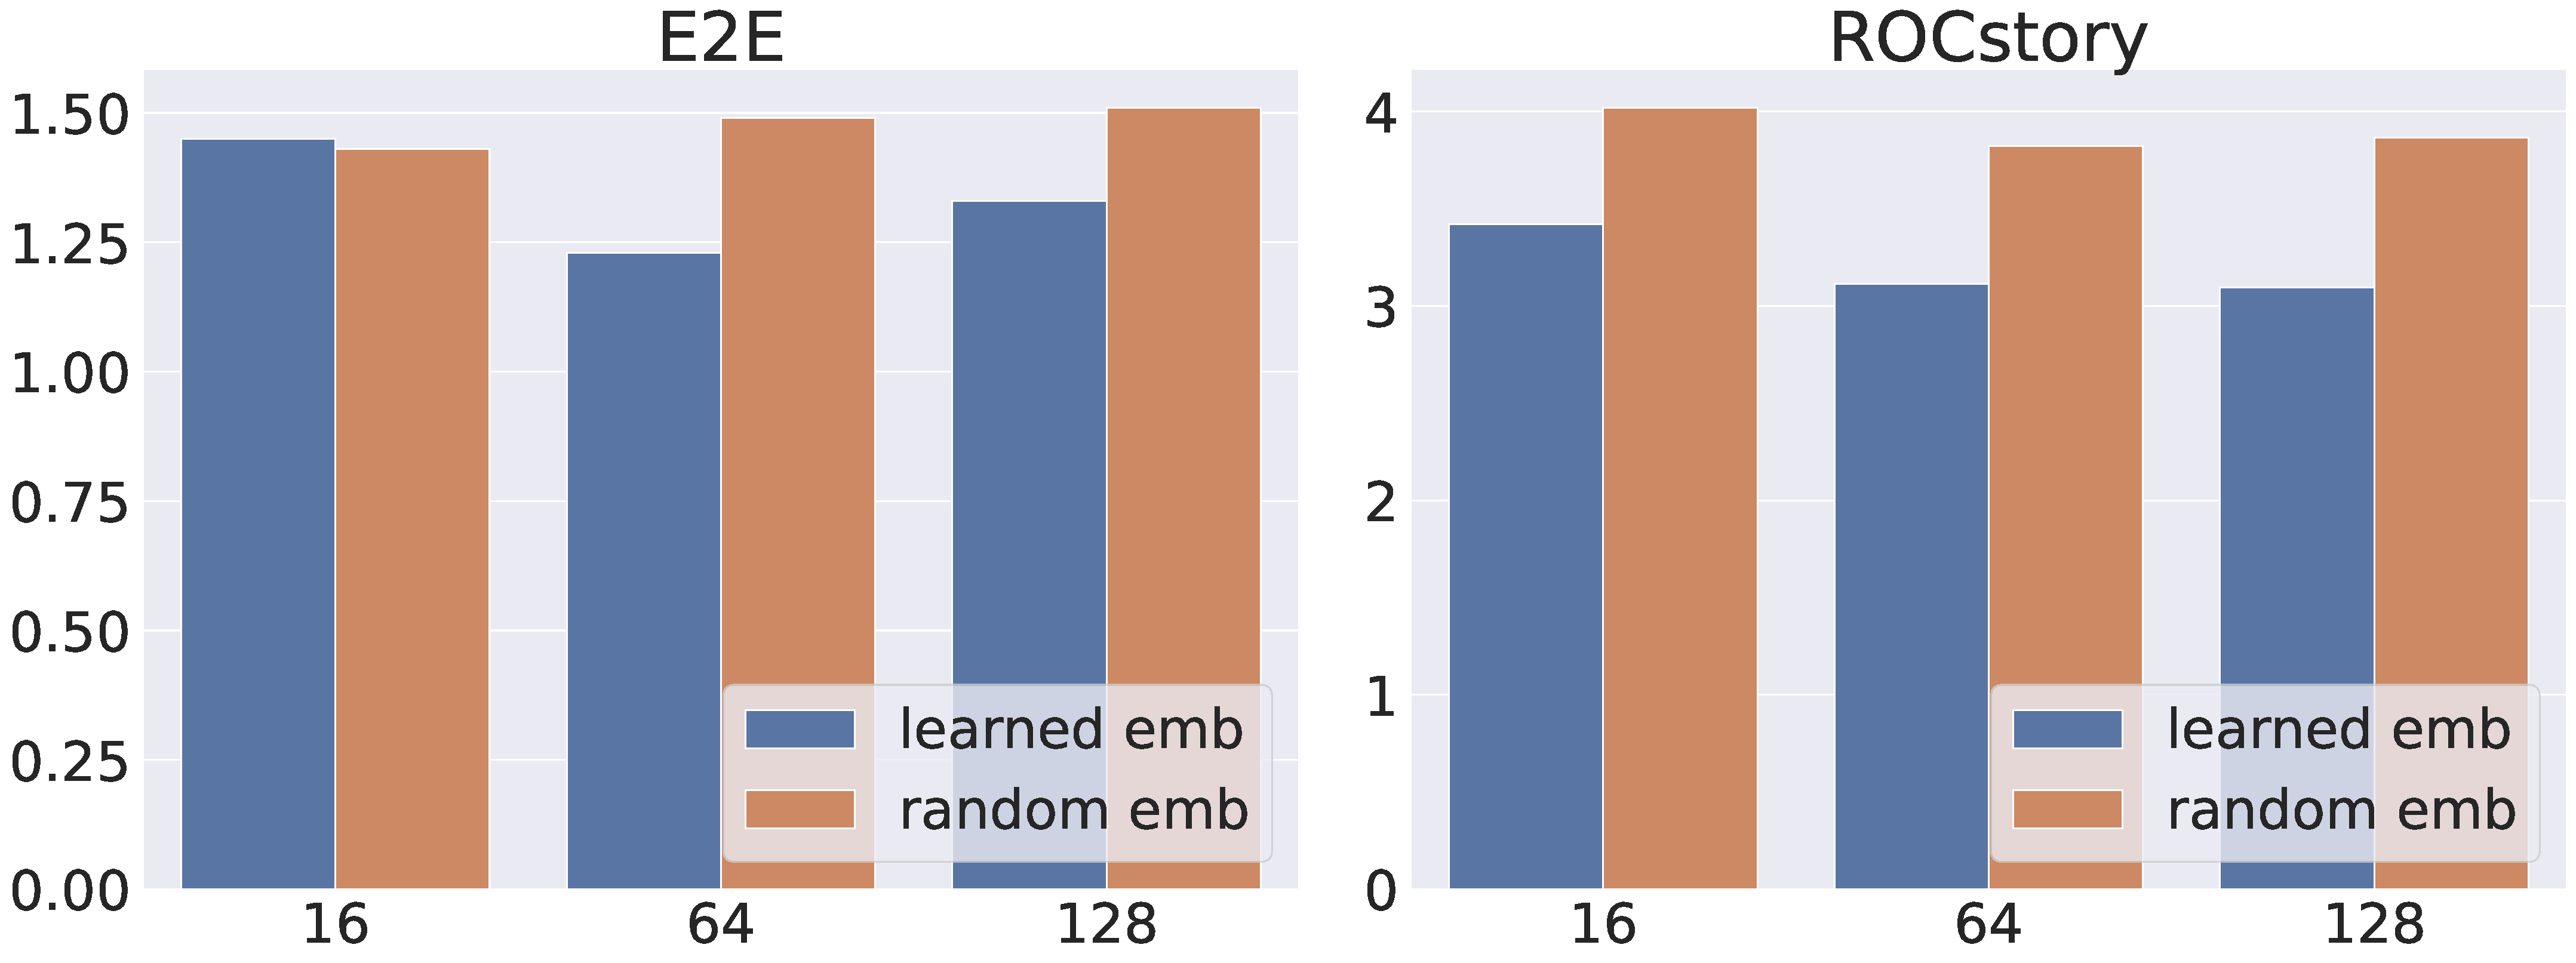
\includegraphics[width=0.8\textwidth]{fig/ablation_emb_e2e_appendix.pdf}
    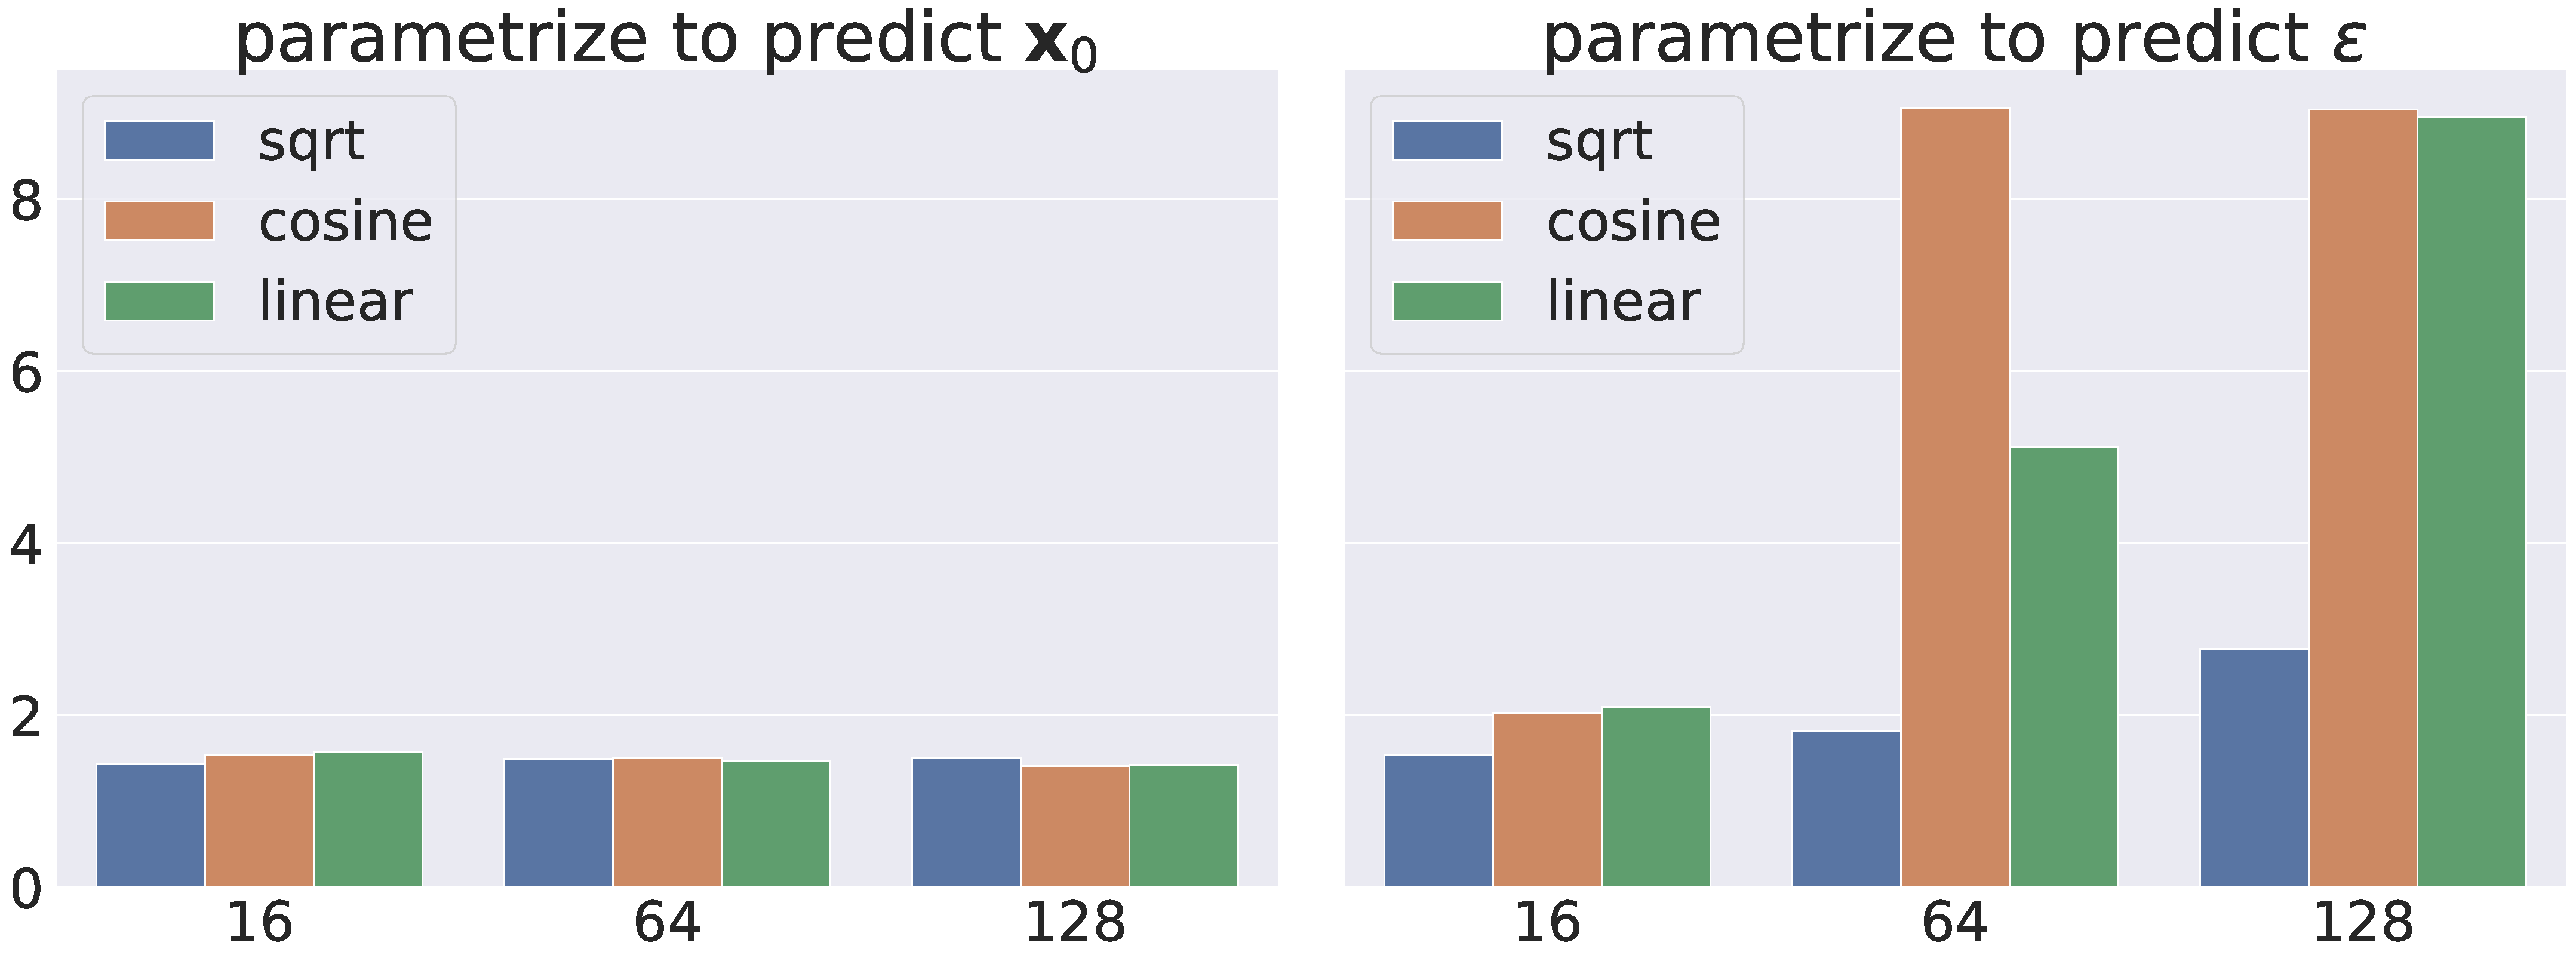
\includegraphics[width=0.8\textwidth]{fig/ablation_parametrization_appendix.pdf}
    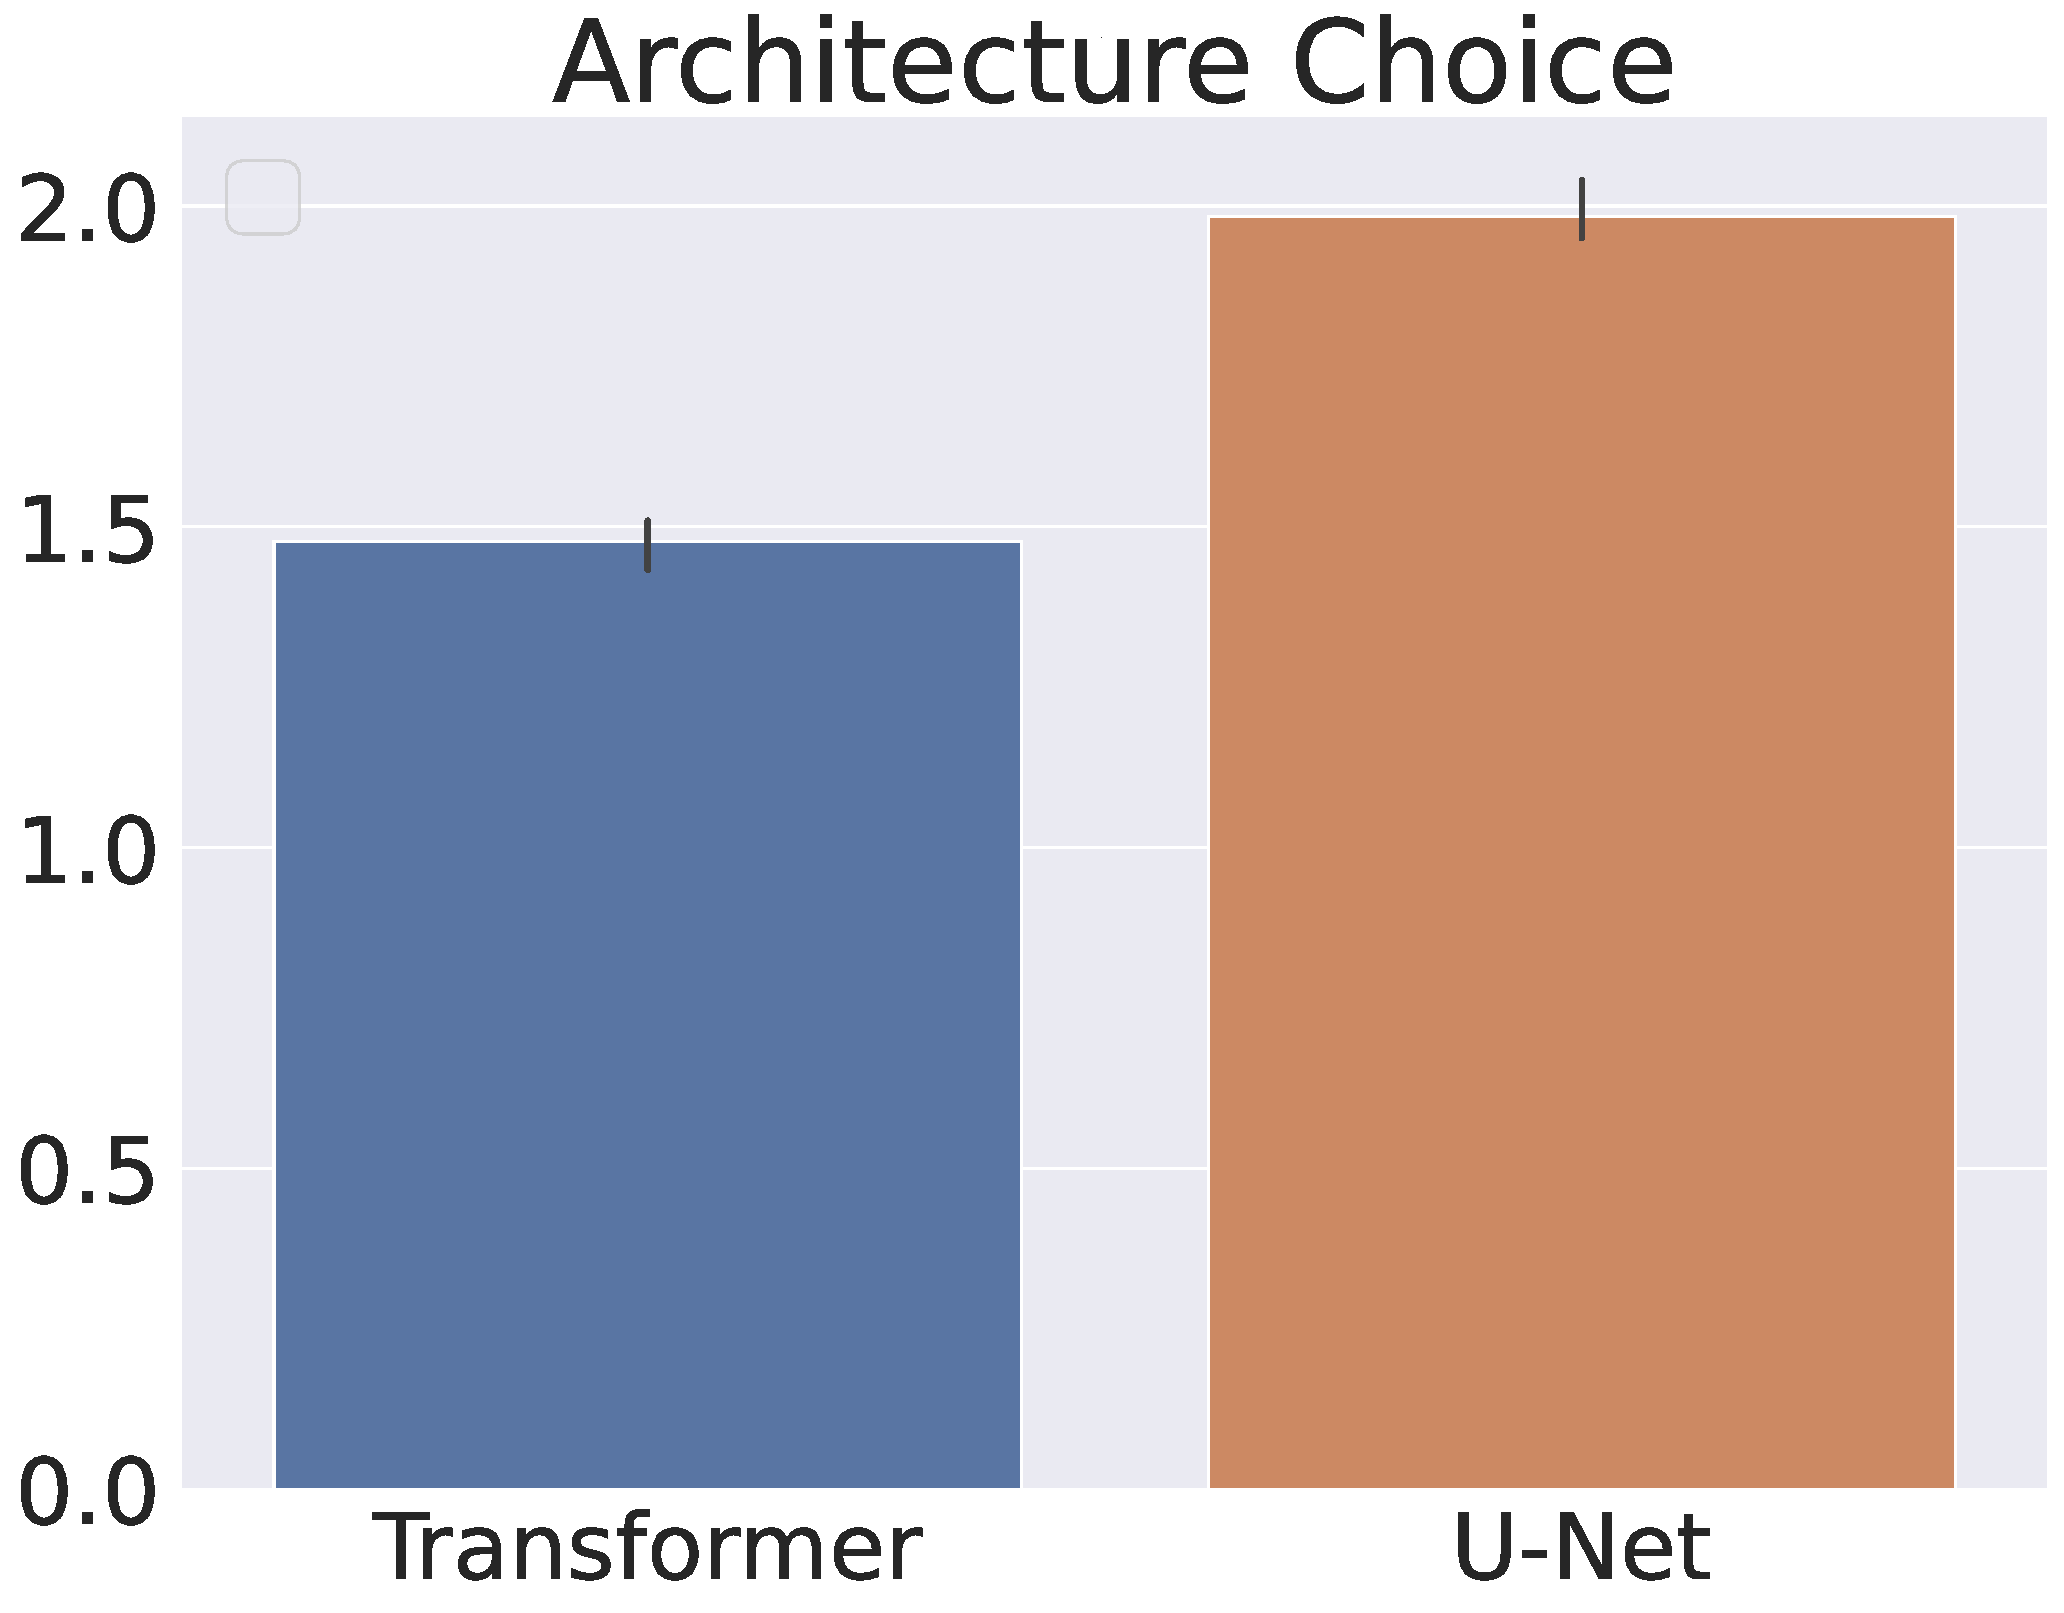
\includegraphics[width=0.4\textwidth]{fig/ablation_architecture_appendix.pdf}
\caption{\label{app:tab:ablation} 附加消融结果。第一行显示，带有可训练 embeddings 的 Diffusion-LM 在两个数据集上都优于随机 embeddings（\cref{ssec:embeddings}）。第二行表明，\sqrtt 调度在所有维度和参数化选择上都取得一致良好且稳定的性能。最后一行显示，对于语言建模，Transformer 架构优于 U-Net 架构。
}
\end{figure}


\section{社会影响}
一方面，语言模型具备强可控性将有助于缓解毒性，使语言模型的部署更加可靠。此外，我们还可以控制模型更加真实，通过仔细控制其真实性来减少语言模型生成的不准确信息。
然而另一方面，也可以想象，细粒度可控性可能带来更强大的定向虚假信息（例如 narrative wedging）。

为此，值得考虑能够在不影响生成输出流畅性的情况下为其添加水印的生成方法；这类水印也可以被表述为可控生成问题，其中可区分性和流畅性作为约束。

\FloatBarrier

\begin{table*}
    \centering
    \resizebox{1\linewidth}{!}{
    \begin{tabular}{lp{13cm}}
\toprule
\parbox[t]{2mm}{\multirow{5}{*}{\rotatebox[origin=c]{90}{ROCStories+Aug}}} & Matt was at the store . He was looking at a new toothbrush . He found the perfect one . When he got home , he bought it . It was bright and he loved it . \\\\
& I and my friend were hungry . We were looking for some to eat . We went to the grocery store . We bought some snacks . We decided to pick up some snacks . \\\\
& I was at the store . I had no money to buy milk . I decided to use the restroom . I went to the register . I was late to work . \\\\
& The man wanted to lose weight . He did n't know how to do weight . He decided to start walking . He ate healthy and ate less . He lost ten pounds in three months . \\\\
& I went to the aquarium . I wanted to feed something . I ordered a fish . When it arrived I had to find something . I was disappointed .\\
\toprule
\toprule
\parbox[t]{2mm}{\multirow{5}{*}{\rotatebox[origin=c]{90}{ROCStories}}} & Tom was planning a trip to California . He had fun in the new apartment . He was driving , until it began to rain . Unfortunately , he was soaked . Tom stayed in the rain at the beach . \\\\
& Carrie wanted a new dress . She did not have enough money . She went to the bank to get one , but saw the missed . Finally , she decided to call her mom . She could not wait to see her new dress . \\\\
& Tina went to her first football game . She was excited about it . When she got into the car she realized she forgot her hand . She ended up getting too late . Tina had to start crying . \\\\
& Michael was at the park . Suddenly he found a stray cat . He decided to keep the cat . He went to his parents and demanded a leg . His parents gave him medicine to get it safe . \\\\
& Tim was eating out with friends . They were out of service . Tim decided to have a pizza sandwich . Tim searched for several hours . He was able to find it within minutes . \\
\toprule
\toprule
\parbox[t]{2mm}{\multirow{5}{*}{\rotatebox[origin=l]{90}{E2E}}} 
& The Waterman is an expensive pub that serves Japanese food . It is located in Riverside and has a low customer rating . \\\\
& A high priced pub in the city centre is The Olive Grove . It is a family friendly pub serving French food . \\\\
& The Rice Boat offers moderate priced Chinese food with a customer rating of 3 out of 5 . It is near Express by Holiday Inn . \\\\
& There is a fast food restaurant , The Phoenix , in the city centre . It has a price range of more than \u00a3 30 and the customer ratings are low .\\\\
& The Mill is a coffee shop based in the city centre area near to The Sorrento . It is in the high price range and serves Indian food . \\
\bottomrule
    \end{tabular}}
\caption{\label{app:qualitative-unc} 由在 3 个数据集上训练的 Diffusion-LM 通过无条件采样生成的随机示例。ROCStories+Aug 表示带数据增强的 ROCStories。它通过先在 ROCStories 数据集上微调 GPT-j，再采样大型 GPT-j 模型生成 1M 个故事而得到。}
\end{table*}


\begin{table*}
    \centering
    \resizebox{0.95\linewidth}{!}{
    \begin{tabular}{lp{13cm}}
\toprule
target span & [3, 5, PP] \\ 
\midrule
FUDGE &  UNK the UNK \greenspan{for Italian food} , The Eagle coffee shop is near Burger King in the riverside area . The Eagle has a customer rating of 5 out of 5 , and isn ' t family - friendly . The Eagle has a cheap price range . \\
Diffusion-LM &   The Plough , \greenspan{near Café Rouge} , is a high priced fast food pub . \\
FT &  Along the riverside \greenspan{near Café Rouge} is The Golden Curry . It serves Italian food in a family - friendly environment . It has a low customer rating . \\
\toprule
target span & [10, 12, PP]\\
\midrule
FUDGE &  Blue Spice is a high price range Fast food located \greenspan{in city centre} .\\
Diffusion-LM &   The Phoenix is a high priced food restaurant , located \greenspan{near the river} .\\
FT &  The Punter is a family restaurant with low prices and \errorspan{delicious sushi ,} located near the Café Sicilia \\
\toprule
target span & [9, 14, S]\\
\midrule
FUDGE & Zizzi pub serves Italian food for adults only . \errorspan{It has been rated average by} customers . \\
Diffusion-LM &  There is a Chinese restaurant called The Eagle , \greenspan{it has an average customer rating} . \\
FT & On the riverside area are located Alimentum , has \errorspan{a very good French food for} adults and kids , UNK price range are over 20 to 25 £ . \\
\toprule
target span & [4, 16, VP]\\
\midrule
FUDGE & The Cambridge Blue pub \errorspan{is near the Café Brazil and offers a high price range for their} French food . \\
Diffusion-LM & On the Ranch there \greenspan{is a children friendly pub called The Cricketers with an average customer rating} . \\
FT &  The Travellers Rest Beefeater \greenspan{is an average rated restaurant located in the riverside area near Café Adriatic} . Their price range is less than £ 20 . \\
\toprule
target span & [0, 2, NP]\\
\midrule
FUDGE & \greenspan{The Golden Palace} is a cheap , 5 - star coffee shop , located on the river in the north of the city centre . \\
Diffusion-LM & \greenspan{The Olive Grove} is a pub that provides Indian food in the high price range . It is in the city centre . \\
FT &  \greenspan{The Golden Curry} is located in city centre near Café Rouge which provides English food . Its customer rating is average and is not family - friendly . \\
\toprule
target span & [12, 13, NP]\\
\midrule
FUDGE & The Waterman is a family friendly place with a good rating .\errorspan{ [missing span]}\\
Diffusion-LM &   The Vaults is a high priced , family friendly restaurant that serves \greenspan{Italian food} . \\
FT &  Strada is a restaurant which costs less than £ 20 , but \errorspan{is not} family - friendly and has an average rating . \\
 
\bottomrule
\end{tabular}}
\caption{\label{app:qualitative-span} syntax span 控制任务的定性输出。目标 span（$i,j,$label）表示从位置 $i$ 到位置 $j$ 的 span 应是具有特定标签的成分：S 是 sentence，NP 是 noun phrase，VP 是 verb phrase，PP 是 prepositional phrase，等等。我们将\errorspan{失败 spans 标为红色}，将\greenspan{正确 spans 标为绿色}。}
\end{table*}



\begin{table*}
    \centering
    \resizebox{0.95\linewidth}{!}{
    \begin{tabular}{lp{13cm}}
\toprule
target POS &  PROPN AUX DET ADJ NOUN NOUN VERB ADP DET NOUN ADP DET NOUN PUNCT\\
\midrule
FUDGE &  Aromi is a non family - friendly fast food coffee shop in the riverside area with a low Customer Rating . \\
Diffusion-LM &   Fitzbillies is a cheap coffee shop located on the outskirts of the city . \\
FT &  Aromi is a fast food pub located at the centre of the city. 
\\
\toprule
target POS &  PROPN AUX DET NOUN VERB NOUN ADJ NOUN PUNCT PRON NOUN NOUN AUX ADJ\\
\midrule
FUDGE &  Cocum is a family - friendly coffee shop , that has a low price range and a low customer rating . \\
Diffusion-LM &   Zizzi is a pub providing restaurant Chinese food . Its customer rating is low \\
FT &  Zizzi is a pub providing kids friendly services. Its customer rating is average 
\\
\toprule
target POS &  DET NOUN PUNCT PROPN VERB ADJ CCONJ ADJ NOUN CCONJ AUX VERB ADP DET PROPN ADJ PROPN PUNCT\\
\midrule
FUDGE &  A child - friendly coffee shop , Cocum , offers fast food at an average price range of £ 20 - 25 . \\
Diffusion-LM &   The Waterman - friendly serves UNK and fast food and is located near the Crown Plaza Hotel . \\
FT &  The wine - Strada serves fast and cheap food and is located near the Rainbow Vegetarian Café. 
\\
\toprule
target POS &  DET PROPN PROPN VERB ADJ NOUN ADP NOUN ADP SYM NUM PUNCT NOUN NOUN AUX ADJ PUNCT DET PROPN PROPN AUX VERB ADP DET PROPN CCONJ PROPN ADP PROPN PROPN PUNCT ADJ PUNCT DET NOUN PART AUX VERB PUNCT\\
\midrule
FUDGE &  The Midsummer House offers cheap English food near All Bar One . Rated 5 out of 5 . \\
Diffusion-LM &   The Rice Boat provides Chinese food in £ 20 - 25 . Price range is high . The Rice Boat is located near the Express by Holiday Inn and is kids friendly . The customer rating is high . \\
FT &  The Rice Boat welcomes Japanese food with prices under £ 20. Customer ratings are low. The Rice Boat is located near the Express by Holiday Inn. Convenient. No children's are allowed. 
\\
\toprule
target POS &  PROPN PROPN AUX DET ADJ NOUN NOUN ADP DET NOUN NOUN ADP DET PROPN PUNCT PRON AUX NOUN PUNCT ADJ PUNCT\\
\midrule
FUDGE &  Loch Fyne is a Japanese restaurant with a moderate price range and kid - friendly atmosphere . \\
Diffusion-LM &   Browns Cambridge is an Italian restaurant shop in the city centre near The Sorrento . It is family - friendly . \\
FT &  Browns Cambridge is a cheap coffee shop in the riverside area near The Sorrento, that is family - friendly. 
\\
\toprule
target POS &  PROPN VERB DET ADJ NOUN NOUN PROPN PUNCT PRON AUX ADJ VERB CCONJ VERB NOUN SCONJ VERB ADJ NOUN PUNCT\\
\midrule
FUDGE &  Fitzbillies coffee shop has a high price range , children friendly service and serves Japanese food in riverside with high customer rating . \\
Diffusion-LM &   There has a high customer rating . It is kid friendly called The Golden Curry and serves Indian food . \\
FT &  Customers give the French coffee shop Fitzbillies ; it is average rated and offers families where serving light meals. 
\\
\toprule
target POS &  DET NUM NUM VERB ADJ NOUN\\
\midrule
FUDGE &  The Twenty Two serves Fast food and is kids friendly . \\
Diffusion-LM &  The Twenty Two provides Chinese food \\
FT &  The Twenty Two provides Indian food 
\\
\toprule
target POS &  ADV NOUN ADV ADP PROPN PROPN PUNCT DET PROPN NOUN NOUN VERB ADJ NOUN NOUN CCONJ AUX PART VERB NOUN NOUN PUNCT\\
\midrule
FUDGE &  UNK your whole family to The Wrestlers , the best UNK the UNK UNK at the river \\
Diffusion-LM &   Located in riverside near The Sorrento , Browns Cambridge coffee shop serves Japanese food , and is not family - friendly . \\
FT &  Even adults only at Loch Fyne, The Rice Boat coffee shop has moderate price range and does not cater kids age. 
\\
\toprule
target POS &  DET PROPN AUX DET NUM NOUN NOUN NOUN VERB ADP DET PROPN PROPN PUNCT\\
\midrule
FUDGE &  The Eagle is a 3 star coffee shop located near Burger King , north of the City centre that provides low - cost fast food . \\
Diffusion-LM &   The Cricketers is a five star coffee shop located near The Portland Arms . \\
FT &  The Vaults is a one star coffee shop located near the Café Brazil. 
\\

\bottomrule
\end{tabular}}
\caption{\label{app:qualitative-pos} POS 控制任务的定性输出。目标 POS 是生成文本应匹配的 gold parts-of-speech 标签序列。}
\end{table*}


\begin{table*}
    \centering
    \resizebox{0.95\linewidth}{!}{
    \begin{tabular}{lp{13cm}}
\toprule
target length &  7 \\
\midrule
FUDGE &  Wildwood is a cheap Japanese pub . \errorspan{Low rating .} \\
Diffusion-LM &   The Twenty Two serves Indian food . \\
FT &  The Mill is an Indian restaurant . \\
\toprule
target length &  12 \\
\midrule
FUDGE &  The Phoenix is an average Japanese restaurant that is in the City \errorspan{Centre . }\\
Diffusion-LM &   The Twenty Two serves Chinese food and is not family friendly . \\
FT &  Green Man is an average priced restaurant located near All Bar One \\
\toprule
target length &  17 \\
\midrule
FUDGE &  Fitzbillies is an expensive Italian coffee shop in the city centre . It is not child friendly\errorspan{ . .} \\
Diffusion-LM &  The Twenty Two serves Indian food in the city centre . It is not family friendly . \\
FT &  For low - priced food and a family - friendly atmosphere, visit Fitzbillies near Express by \errorspan{ Holiday Inn }
\\
\toprule
target length &  22 \\
\midrule
FUDGE &  The Golden Curry is an English food restaurant located near the Café Rouge in the Riverside area . The customer rating is \errorspan{average . Children are welcome .} \\
Diffusion-LM &   Strada is a fast food pub located near Yippee Noodle Bar and has a customer rating of 3 out of 5 . \\
FT &  There is an Italian kid friendly restaurant in the riverside area near The Sorrento named Browns Cambridge in the riverside area . \\
\toprule
target length &  27 \\
\midrule
FUDGE &  The Olive Grove is an expensive , children friendly , Fast food restaurant in the city centre . \errorspan{[missing 9 words]}\\
Diffusion-LM &   The Eagle is a family friendly coffee shop in the city centre near Burger King . It serves Italian food and has a low customer rating . \\
FT &  A pub in the city centre near Yippee Noodle Bar is named Strada. It serves French food and has a customer rating of 3 out of \errorspan{ 5 }
\\
\toprule
target length &  32 \\
\midrule
FUDGE &  The Golden Curry is a Japanese food restaurant with a high customer Rating , kid friendly and located along the riverside near Café Rouge . \errorspan{[missing 7 words]}\\
Diffusion-LM &   There is a family - friendly coffee shop in the city centre , it is called Zizzi . It is cheap and has a customer rating of 5 out of 5 . \\
FT &  In the city centre is a kids friendly place called Green Man. It has Japanese food and is near All Bar One. It has a price range of £ 20 \errorspan{ - 25 }
\\
\toprule
target length &  37 \\
\midrule
FUDGE &  There is a coffee shop called Fitzbillies which offers French food at cheap prices . It is not family - friendly and has a customer rating of 5 out of 5 . It is in riverside . \\
Diffusion-LM &   The Rice Boat provides Indian food in the moderate price range . It is located in the city centre . It is near Express by Holiday Inn . Its customer rating is 3 out of 5 . \\
FT &  For a family friendly coffee shop that serves Italian food, with a customer rating of 5 out of 5 and a cheap price range, try The Eagle. It is located in the riverside area \errorspan{. }
\\
\bottomrule
\end{tabular}}
\caption{\label{app:qualitative-length} 长度控制任务的定性输出，其中所有生成文本都试图精确匹配目标长度。我们将超过目标长度的词标为\errorspan{红色}。}
\end{table*}


\begin{table*}
    \centering
    \resizebox{0.95\linewidth}{!}{
    \begin{tabular}{lp{13cm}}
\toprule
\toprule
target semantic content &  name : Bibimbap House \\
\midrule
FUDGE &  Clare Hall , the \greenspan{Bibimbap House} , serves high end Japanese food in the city centre . \\
Diffusion-LM &   \greenspan{Bibimbap House} in riverside near Clare Hall has a cheap price range . \\
FT &  By Clare Hall is \greenspan{Bibimbap House} which serves expensive noodles. 
\\
\toprule
target semantic content &  name : Travellers Rest Beefeater \\
\midrule
FUDGE &  \errorspan{Clowns} near Clare Hall in riverside is a French coffee shop rated 5 out of 5 \\
Diffusion-LM &   \errorspan{Green Man} is an Italian pub located in the city centre near Café UNK . \\
FT &  \greenspan{Travellers Rest Beefeater} is a reasonably priced restaurant that is family friendly. 
\\
\toprule
target semantic content &  Type : coffee shop \\
\midrule
FUDGE &  Wildwood is a \greenspan{coffee shop} located near Ranch . It is expensive and highly UNK . \\
Diffusion-LM &   The Punter is a high priced \greenspan{coffee shop} located near Café Sicilia that serves Japanese food . It is not family - friendly and has a customer rating of 3 out of 5 . \\
FT &  Located in the riverside area is the \greenspan{coffee shop} Fitzbillies. It has Indian food in the price Range of less than £ 20 and a low customer Rating. It is not family Friendly. 
\\
\toprule
target semantic content &  customer rating : low \\
\midrule
FUDGE &  The Waterman is a fast food restaurant that is family - friendly near the city centre . \errorspan{[missing content]}\\
Diffusion-LM &   The Rice Boat restaurant has a \greenspan{low customer rating} and is located in riverside . It serves Italian food , and is not family - friendly . \\
FT &  The Eagle is \greenspan{low customer rating} coffee shop with Italian food in riverside near Burger King. Its price range is less than £ 20 and is family - friendly. 
\\
\toprule
target semantic content &  near : The Sorrento \\
\midrule
FUDGE &  Browns Cambridge provides Indian food in the less than £ 20 price range . Its customer rating is low . \errorspan{[missing content]}\\
Diffusion-LM &   \greenspan{Near The Sorrento} on the riverside is a pub named Taste of Cambridge that serves Japanese food . \\
FT &  Browns Cambridge sells Italian food and is also a coffee shop. It has an average customer rating. It is located in the riverside area \errorspan{near Crowne Plaza Hotel} and yes it is child friendly. 
\\
\toprule
target semantic content &  food : Italian \\
\midrule
FUDGE &  A non family - friendly \greenspan{Italian} pub is Zizzi . It has an average customer rating .\\
Diffusion-LM &  Loch Fyne is \greenspan{Italian} Japanese restaurant that is kid friendly . \\
FT &   situated near All Bar One is a child friendly \greenspan{Italian} eatery called Green Man costing more than £ 30 is a restaurant near the riverside 
\\
\toprule
target semantic content &  price : high \\
\midrule
FUDGE &  The Vaults is a \greenspan{high priced} Italian Pub with a customer rating of 3 out of 5 near Café Adriatic \\
Diffusion-LM &   The Punter is a French restaurant with a \greenspan{high price} range . \\
FT &  A fast food coffee shop that is not kid friendly is called Cocum. It is \greenspan{expensive} and gets average ratings. 
\\
\end{tabular}}
\caption{\label{app:qualitative-content} 语义内容控制任务的定性输出。我们将符合要求的 spans 标为绿色，将违反控制目标的 spans 标为红色。}
\end{table*}



\end{document}
